\documentclass[../SustainableHEP.tex]{subfiles}
\begin{document}
\RaggedRight
\sloppy
\newpage

%%%%%%%%%%%%%%%%%%%%%%%%%%%%%%%%%%%%%%%%

\section{Resources and Waste}
\label{sec:Waste}

%%%%%%%%%%%%%%%%%%%%%%%%%%%%%%%%%%%%%%%%

\begin{figure}
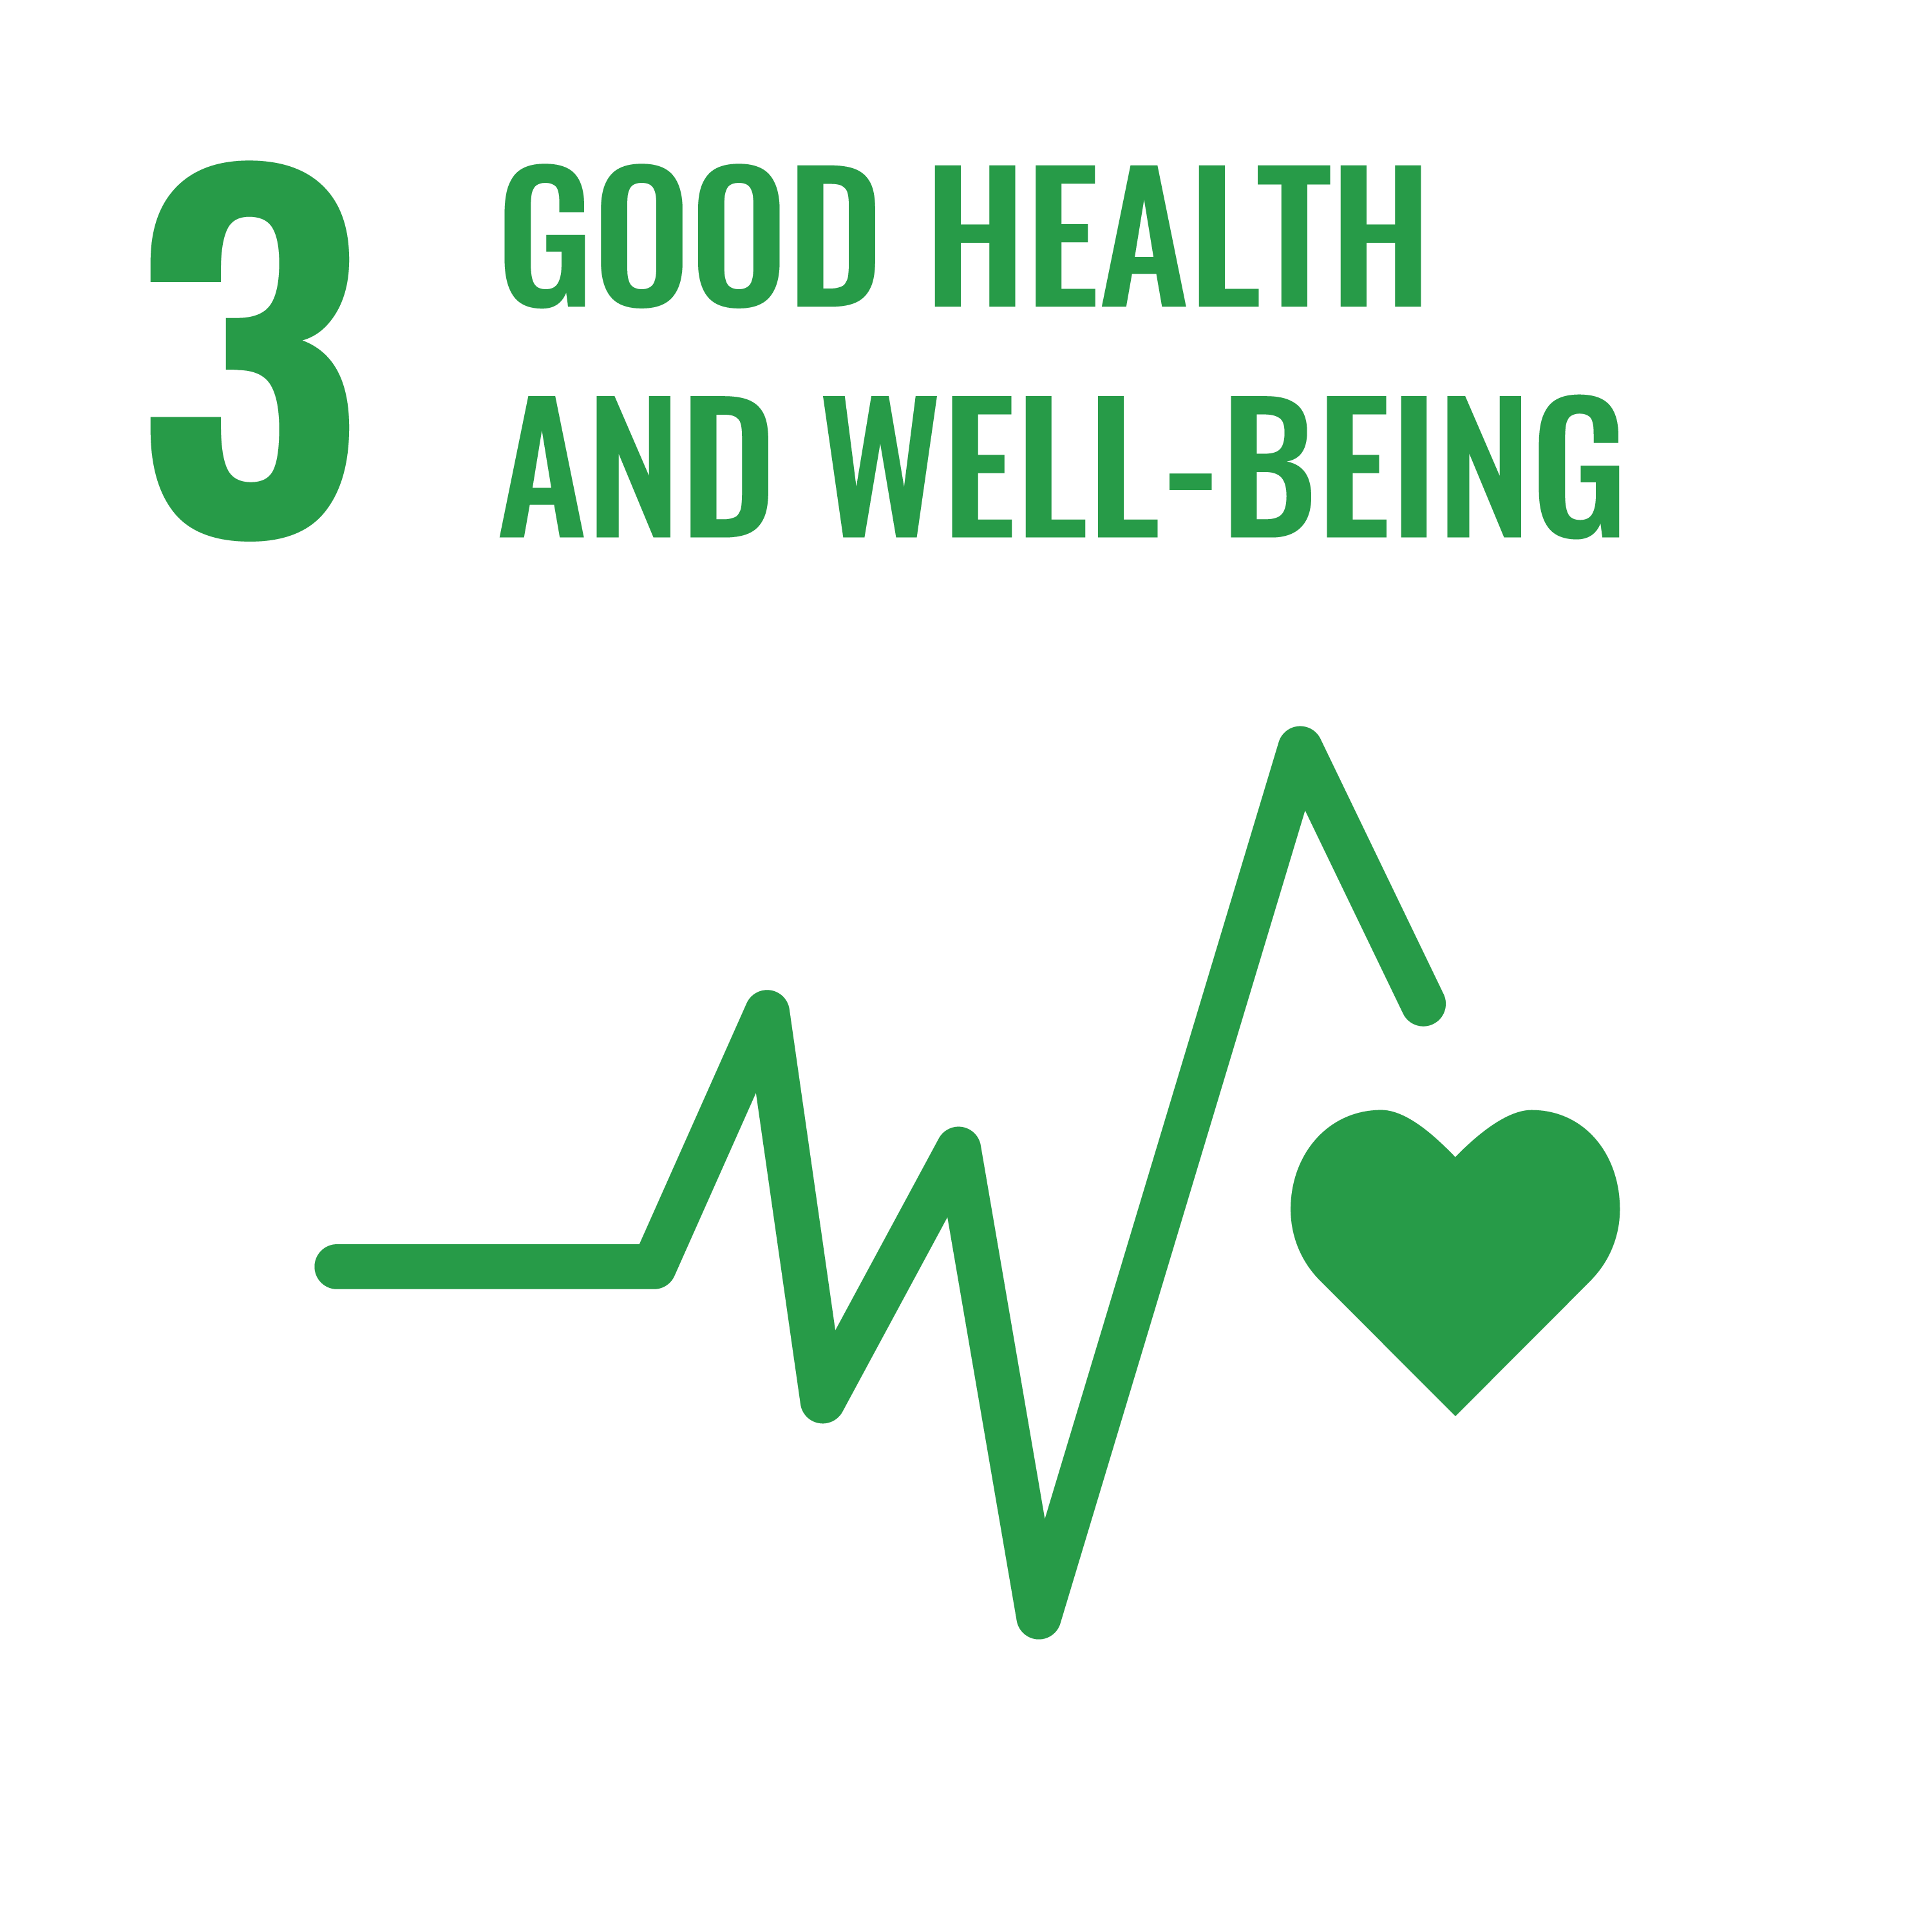
\includegraphics[width=\SDGsize]{Common/SDG_3_GoodHealth.png}~
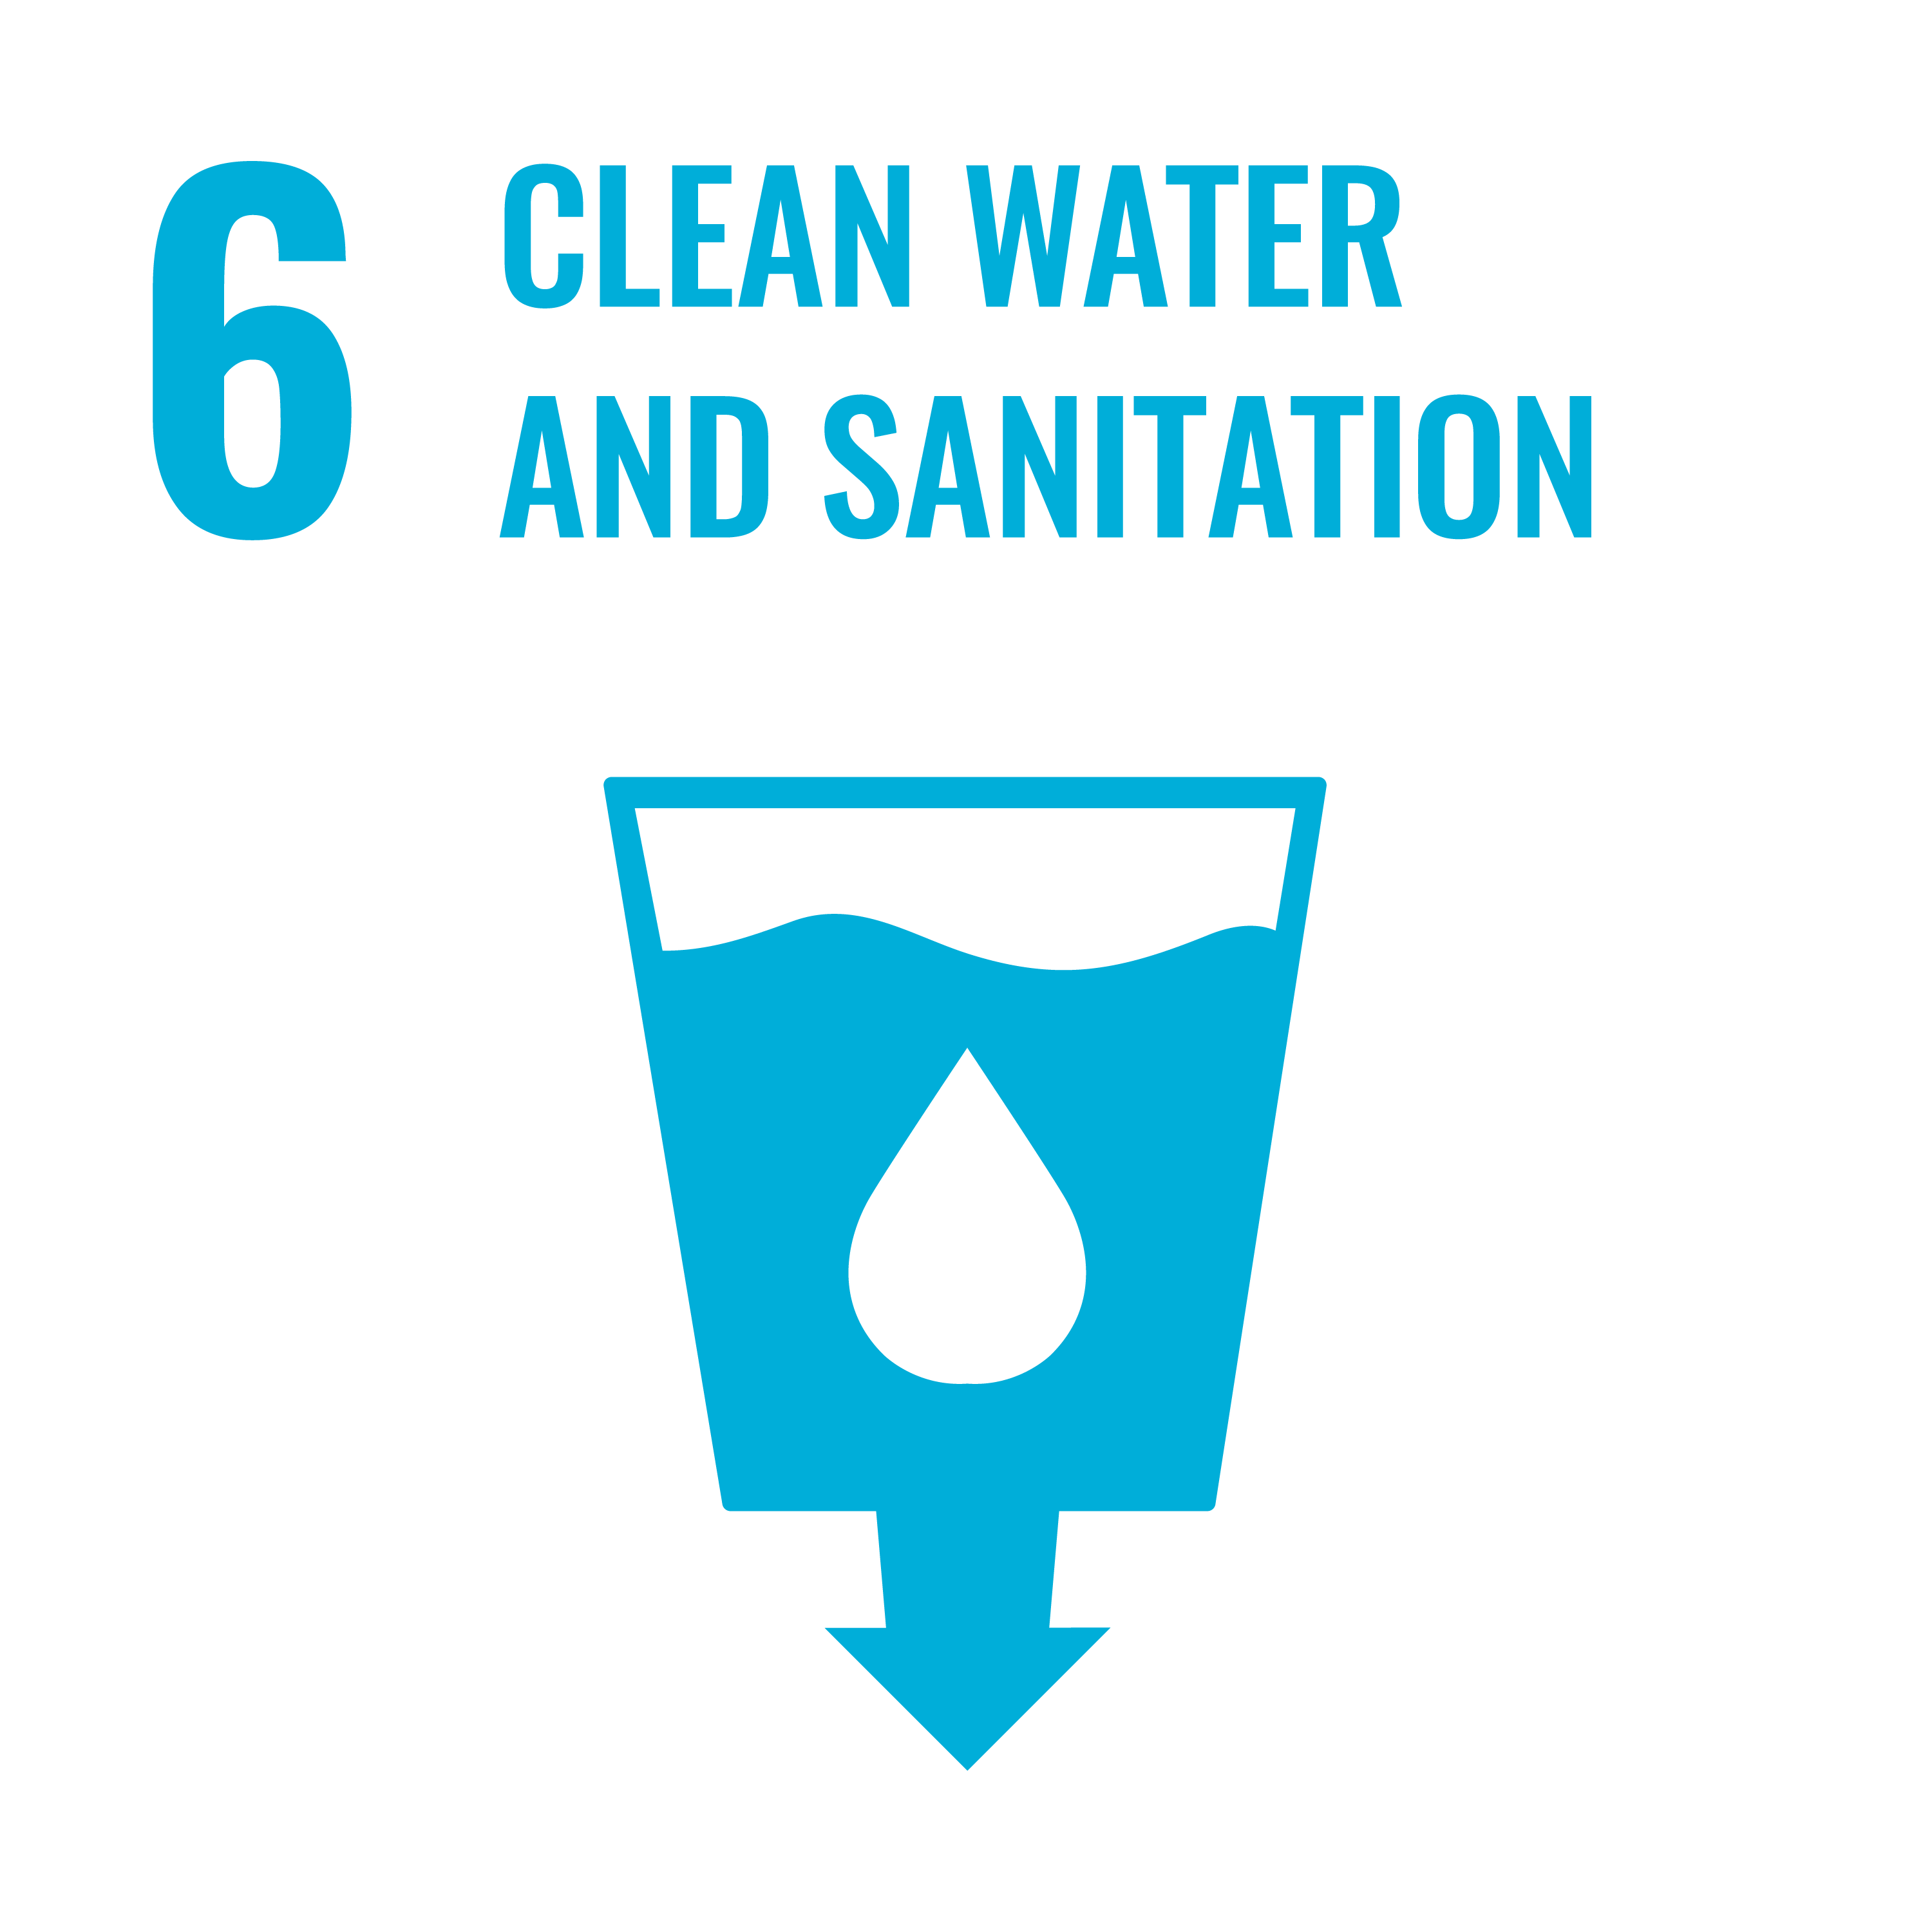
\includegraphics[width=\SDGsize]{Common/SDG_6_CleanWater.png}~
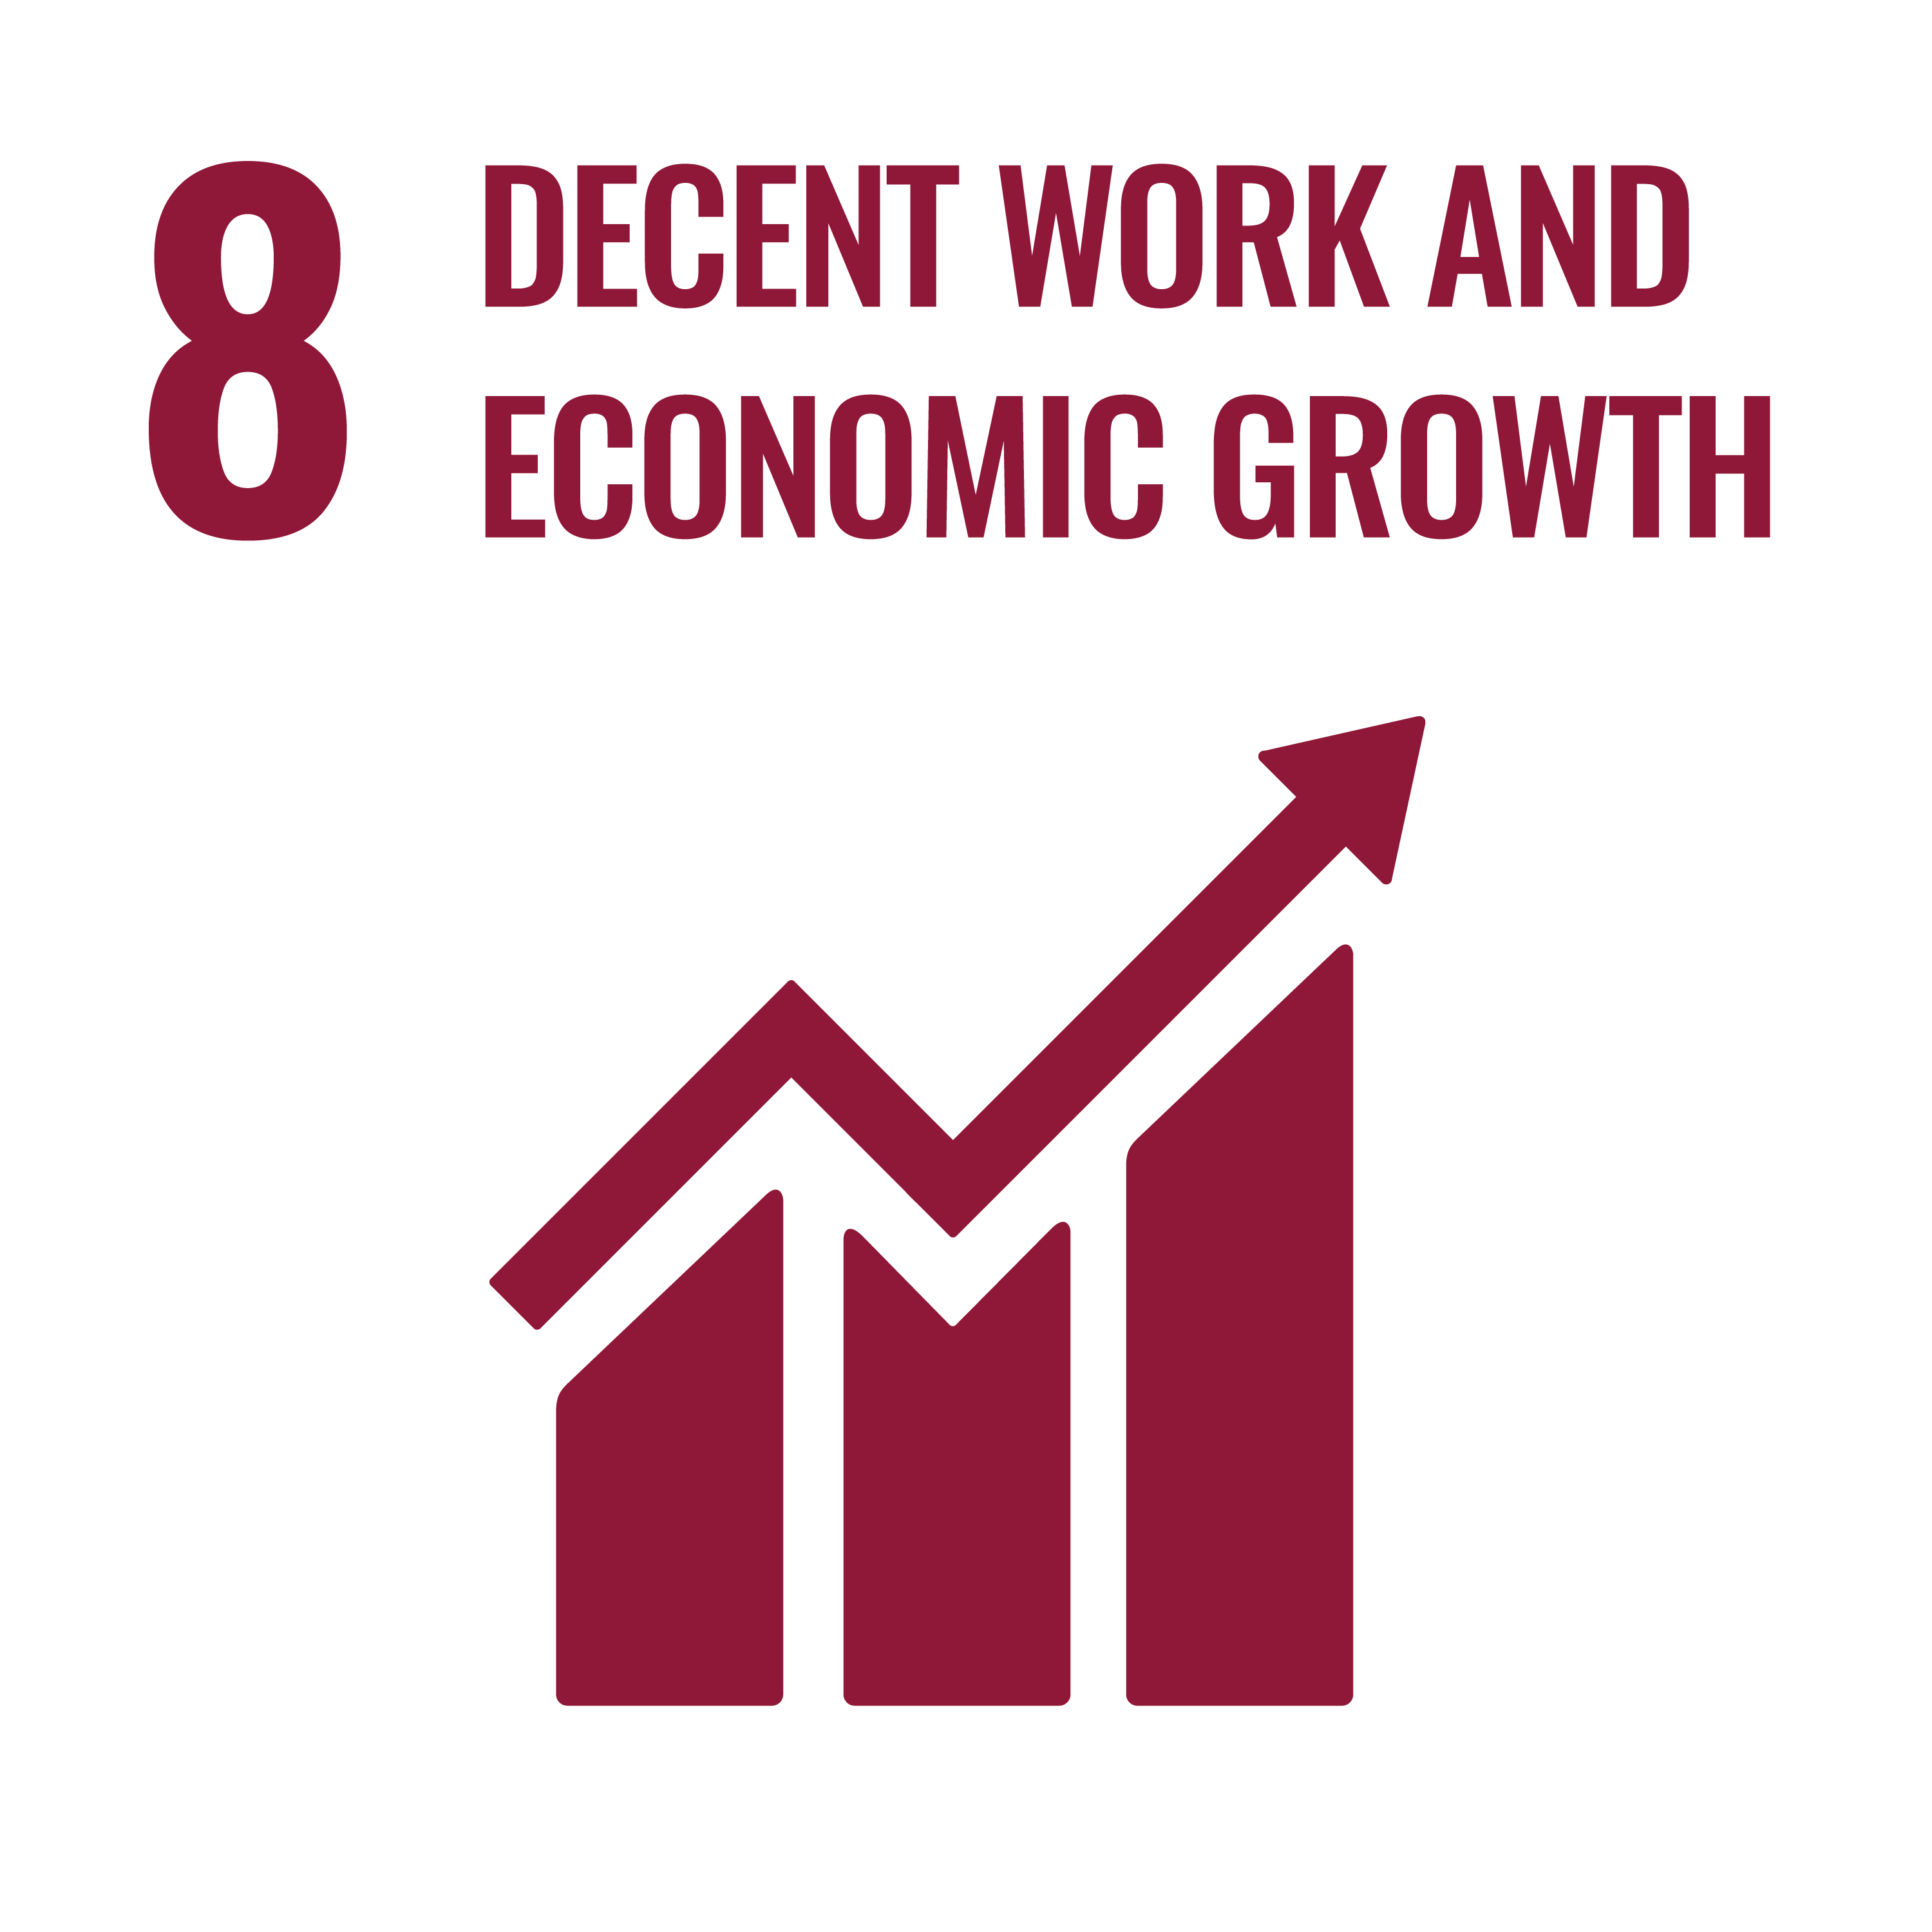
\includegraphics[width=\SDGsize]{Common/SDG_8_EconomicGrowth.png}~
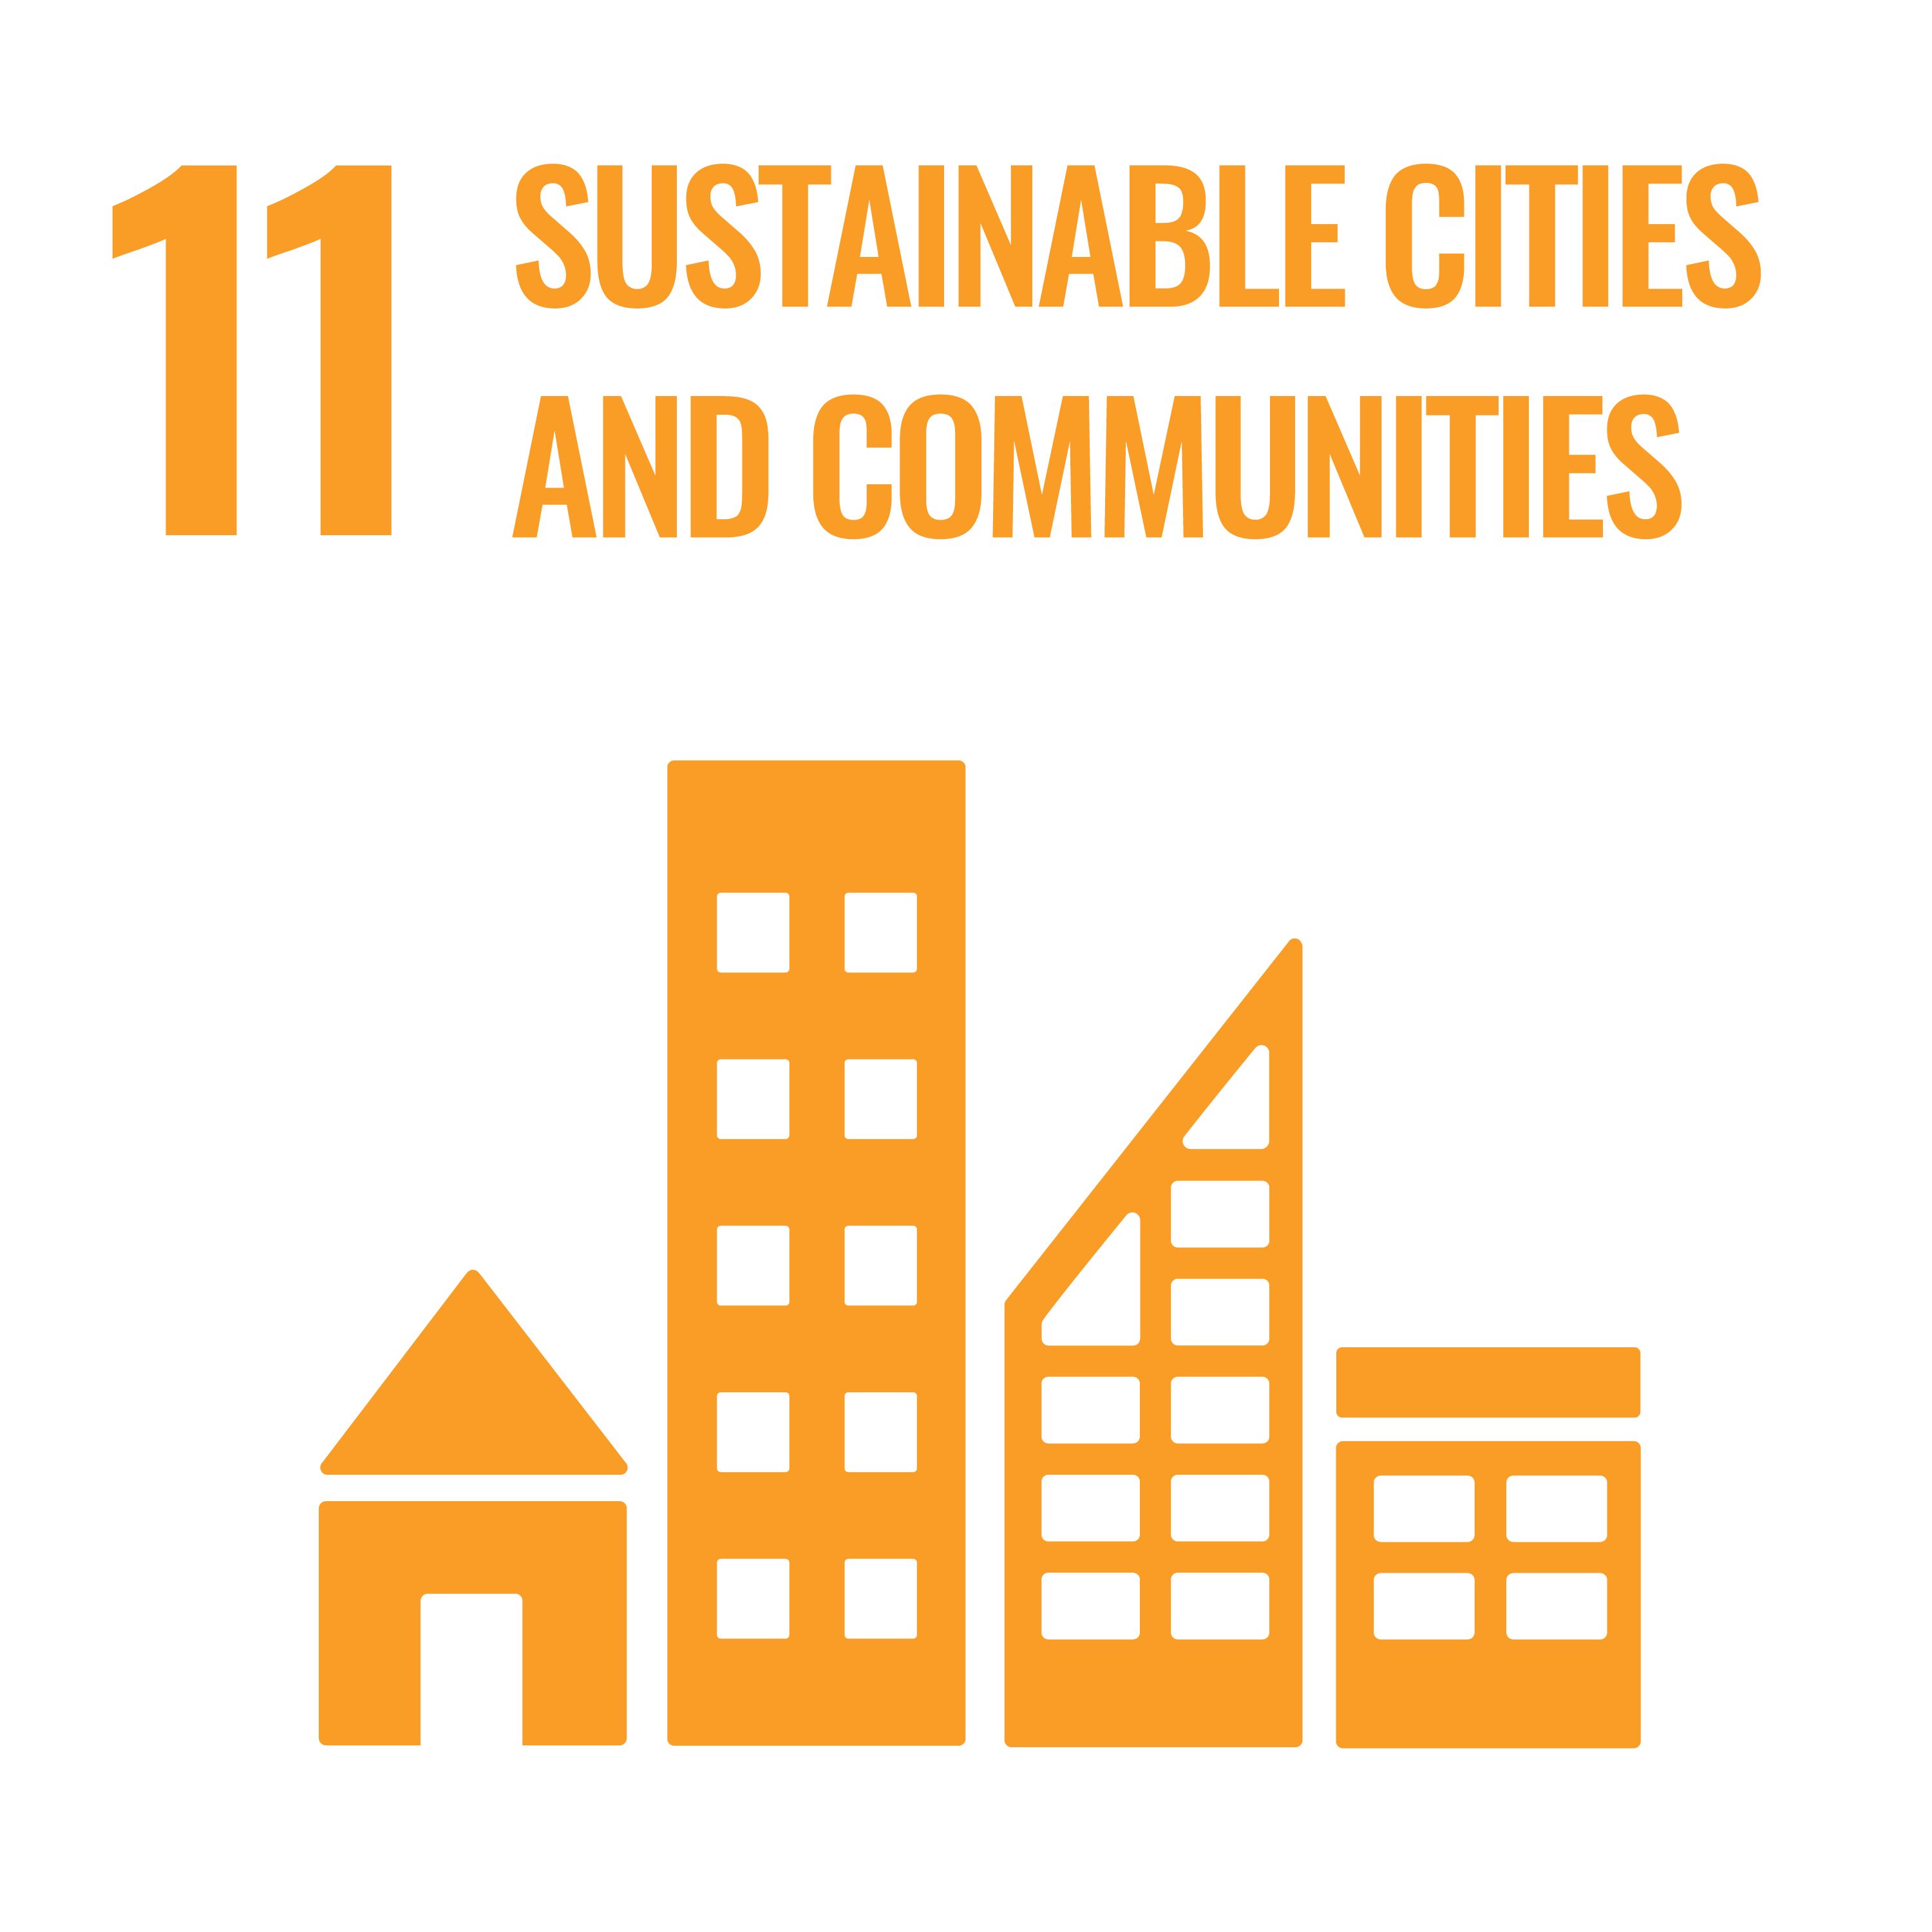
\includegraphics[width=\SDGsize]{Common/SDG_11_SustainableCities.png}~
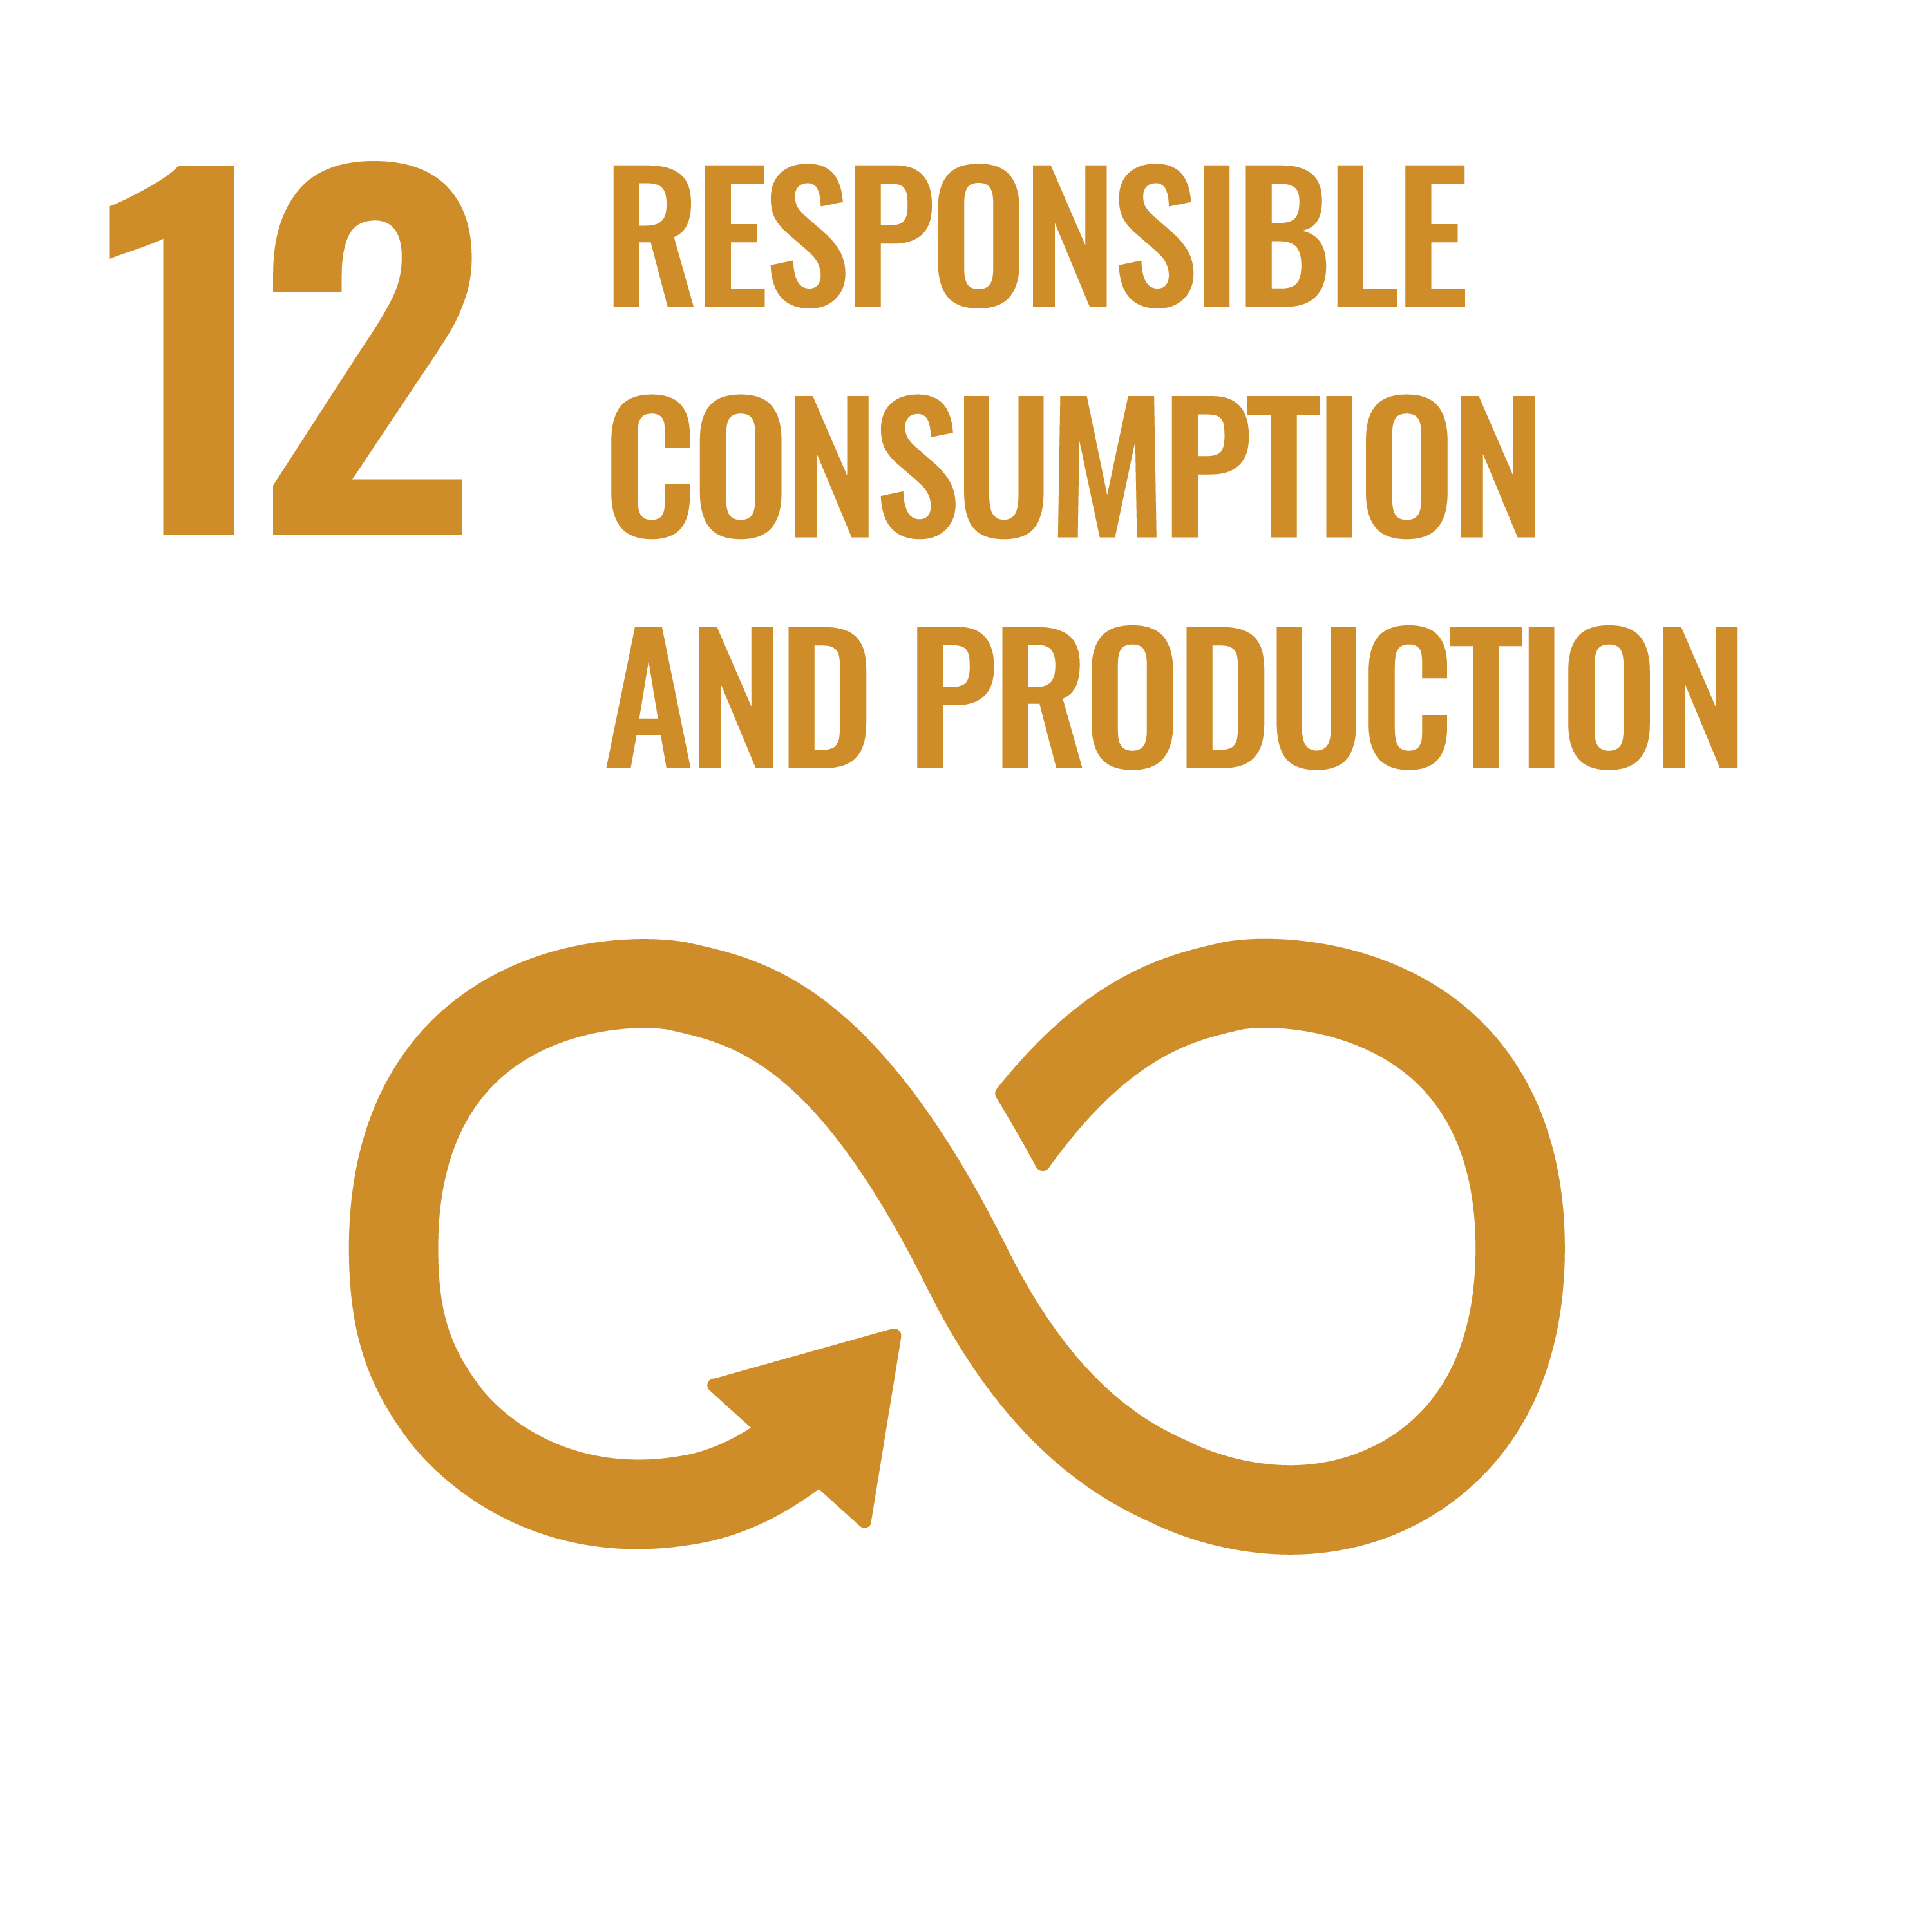
\includegraphics[width=\SDGsize]{Common/SDG_12_ResponsibleConsumption.png}~
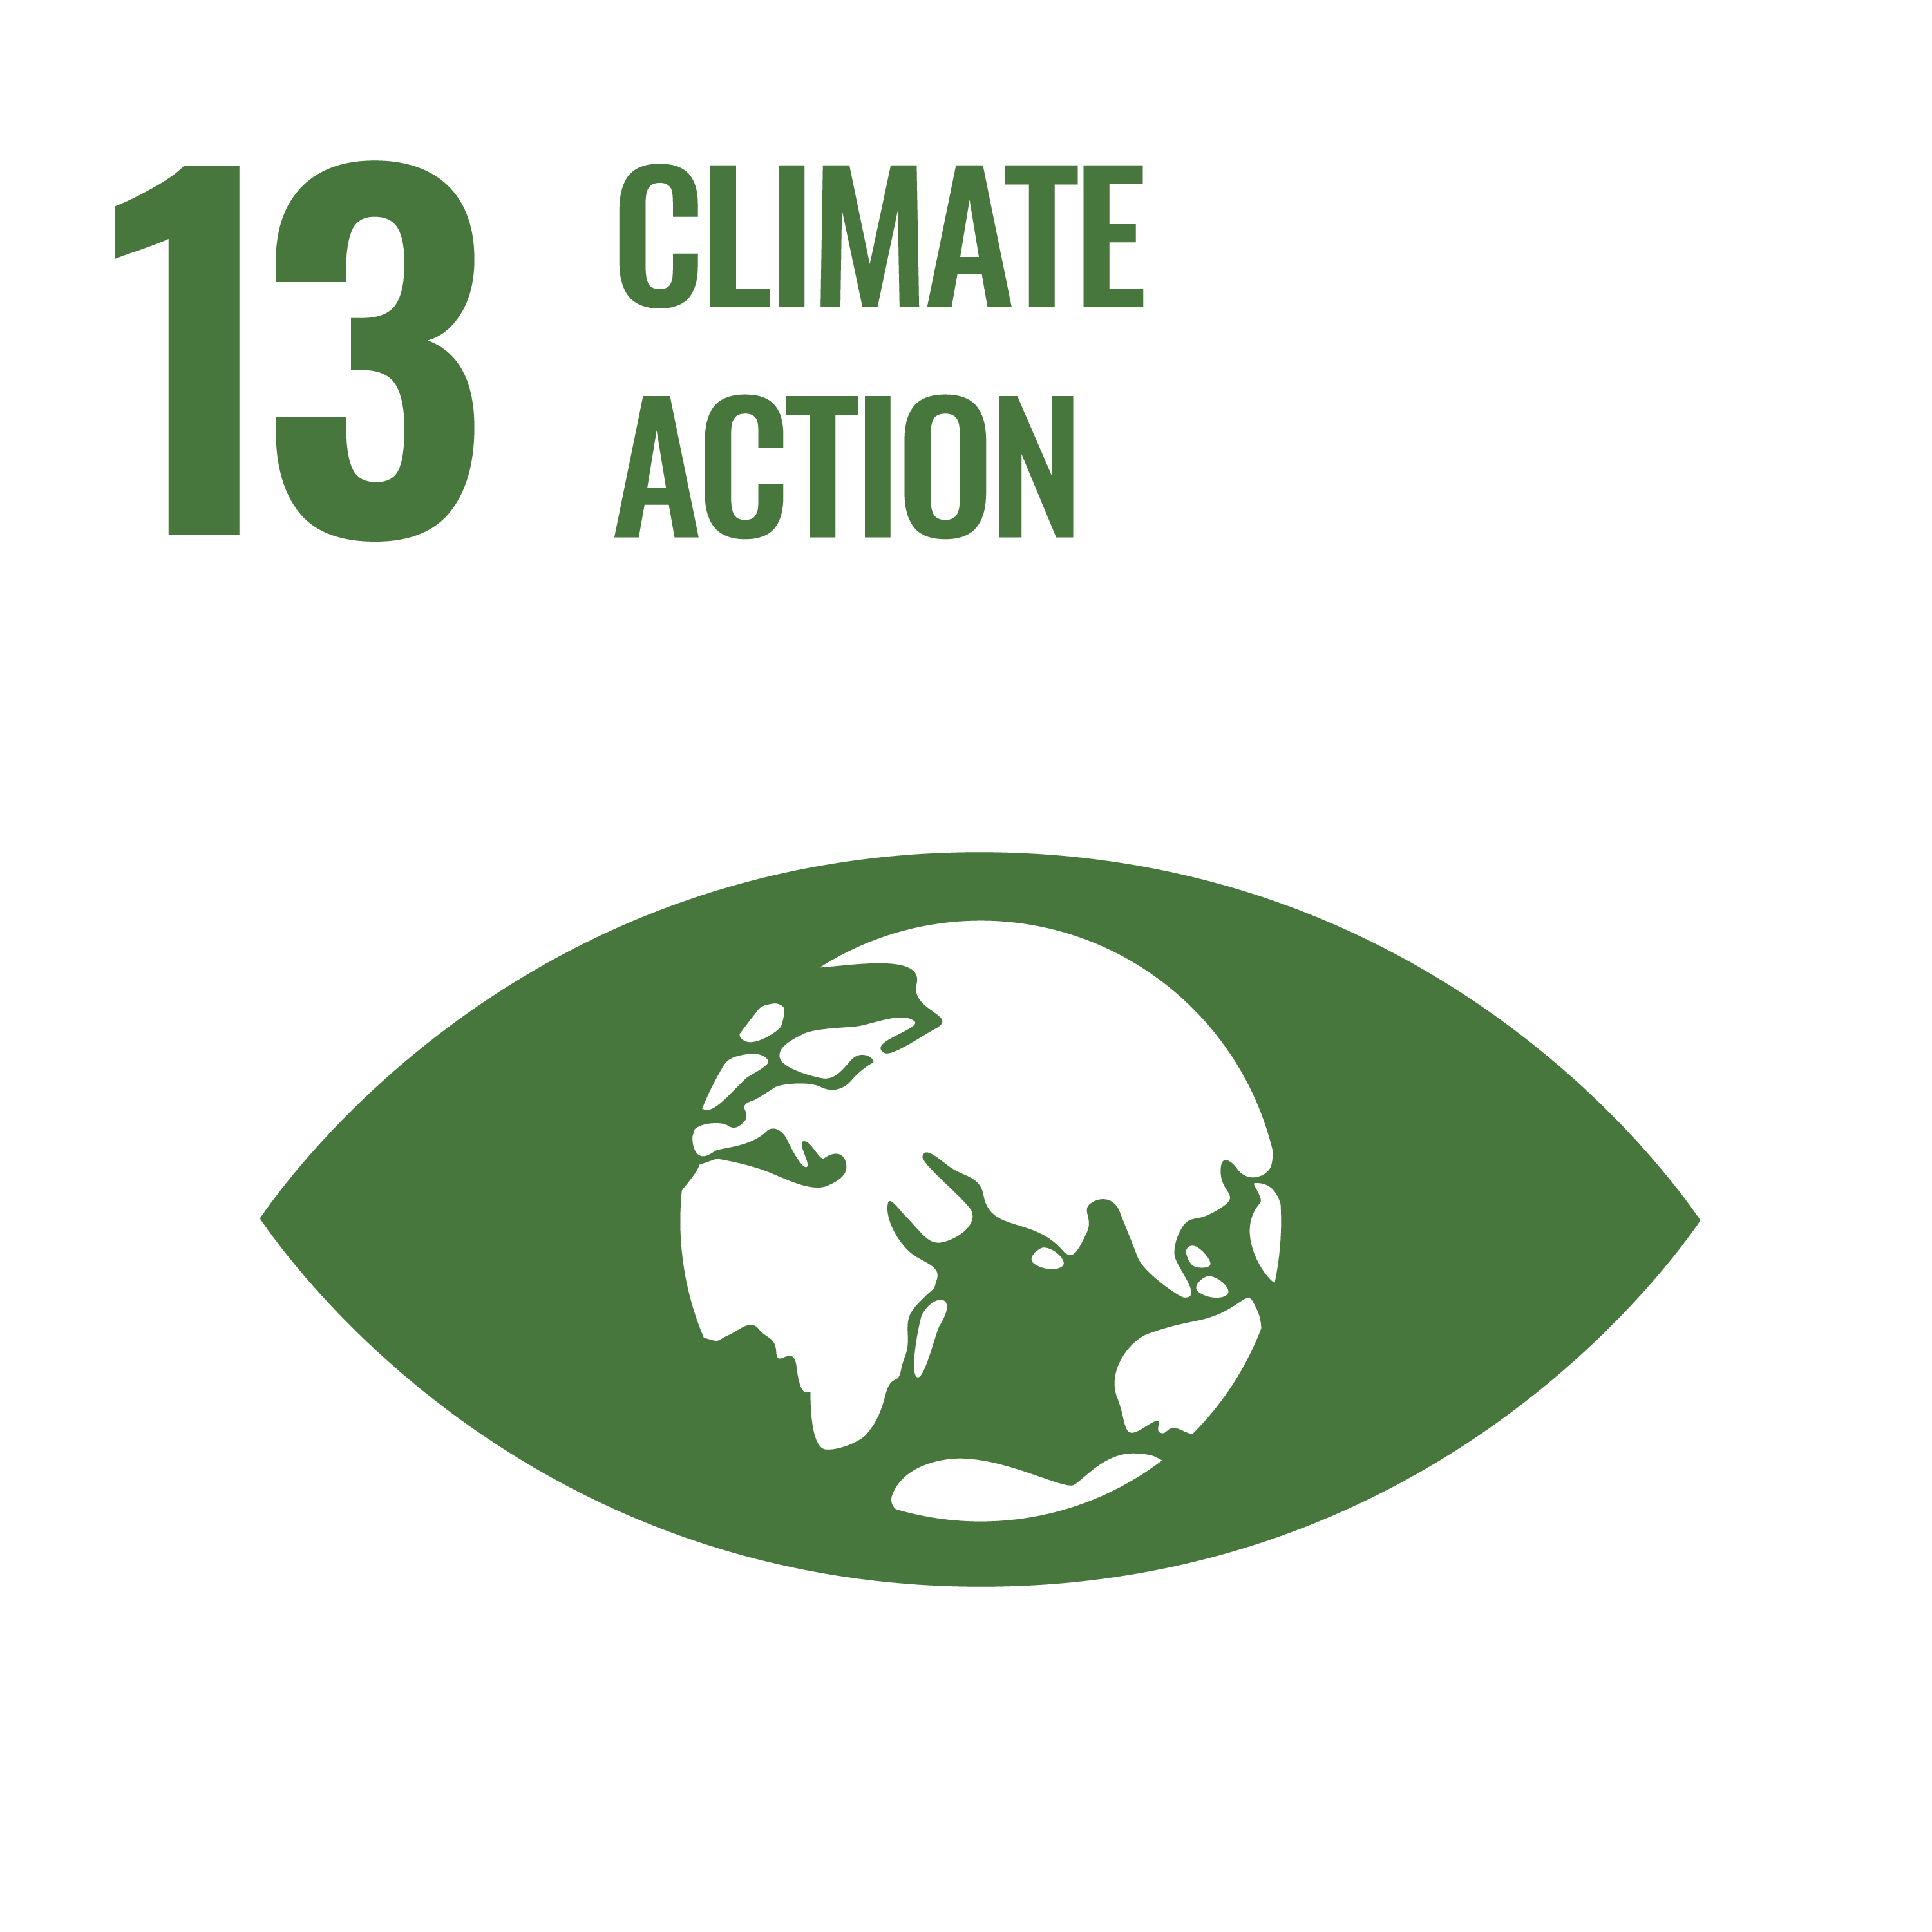
\includegraphics[width=\SDGsize]{Common/SDG_13_ClimateAction.png}~
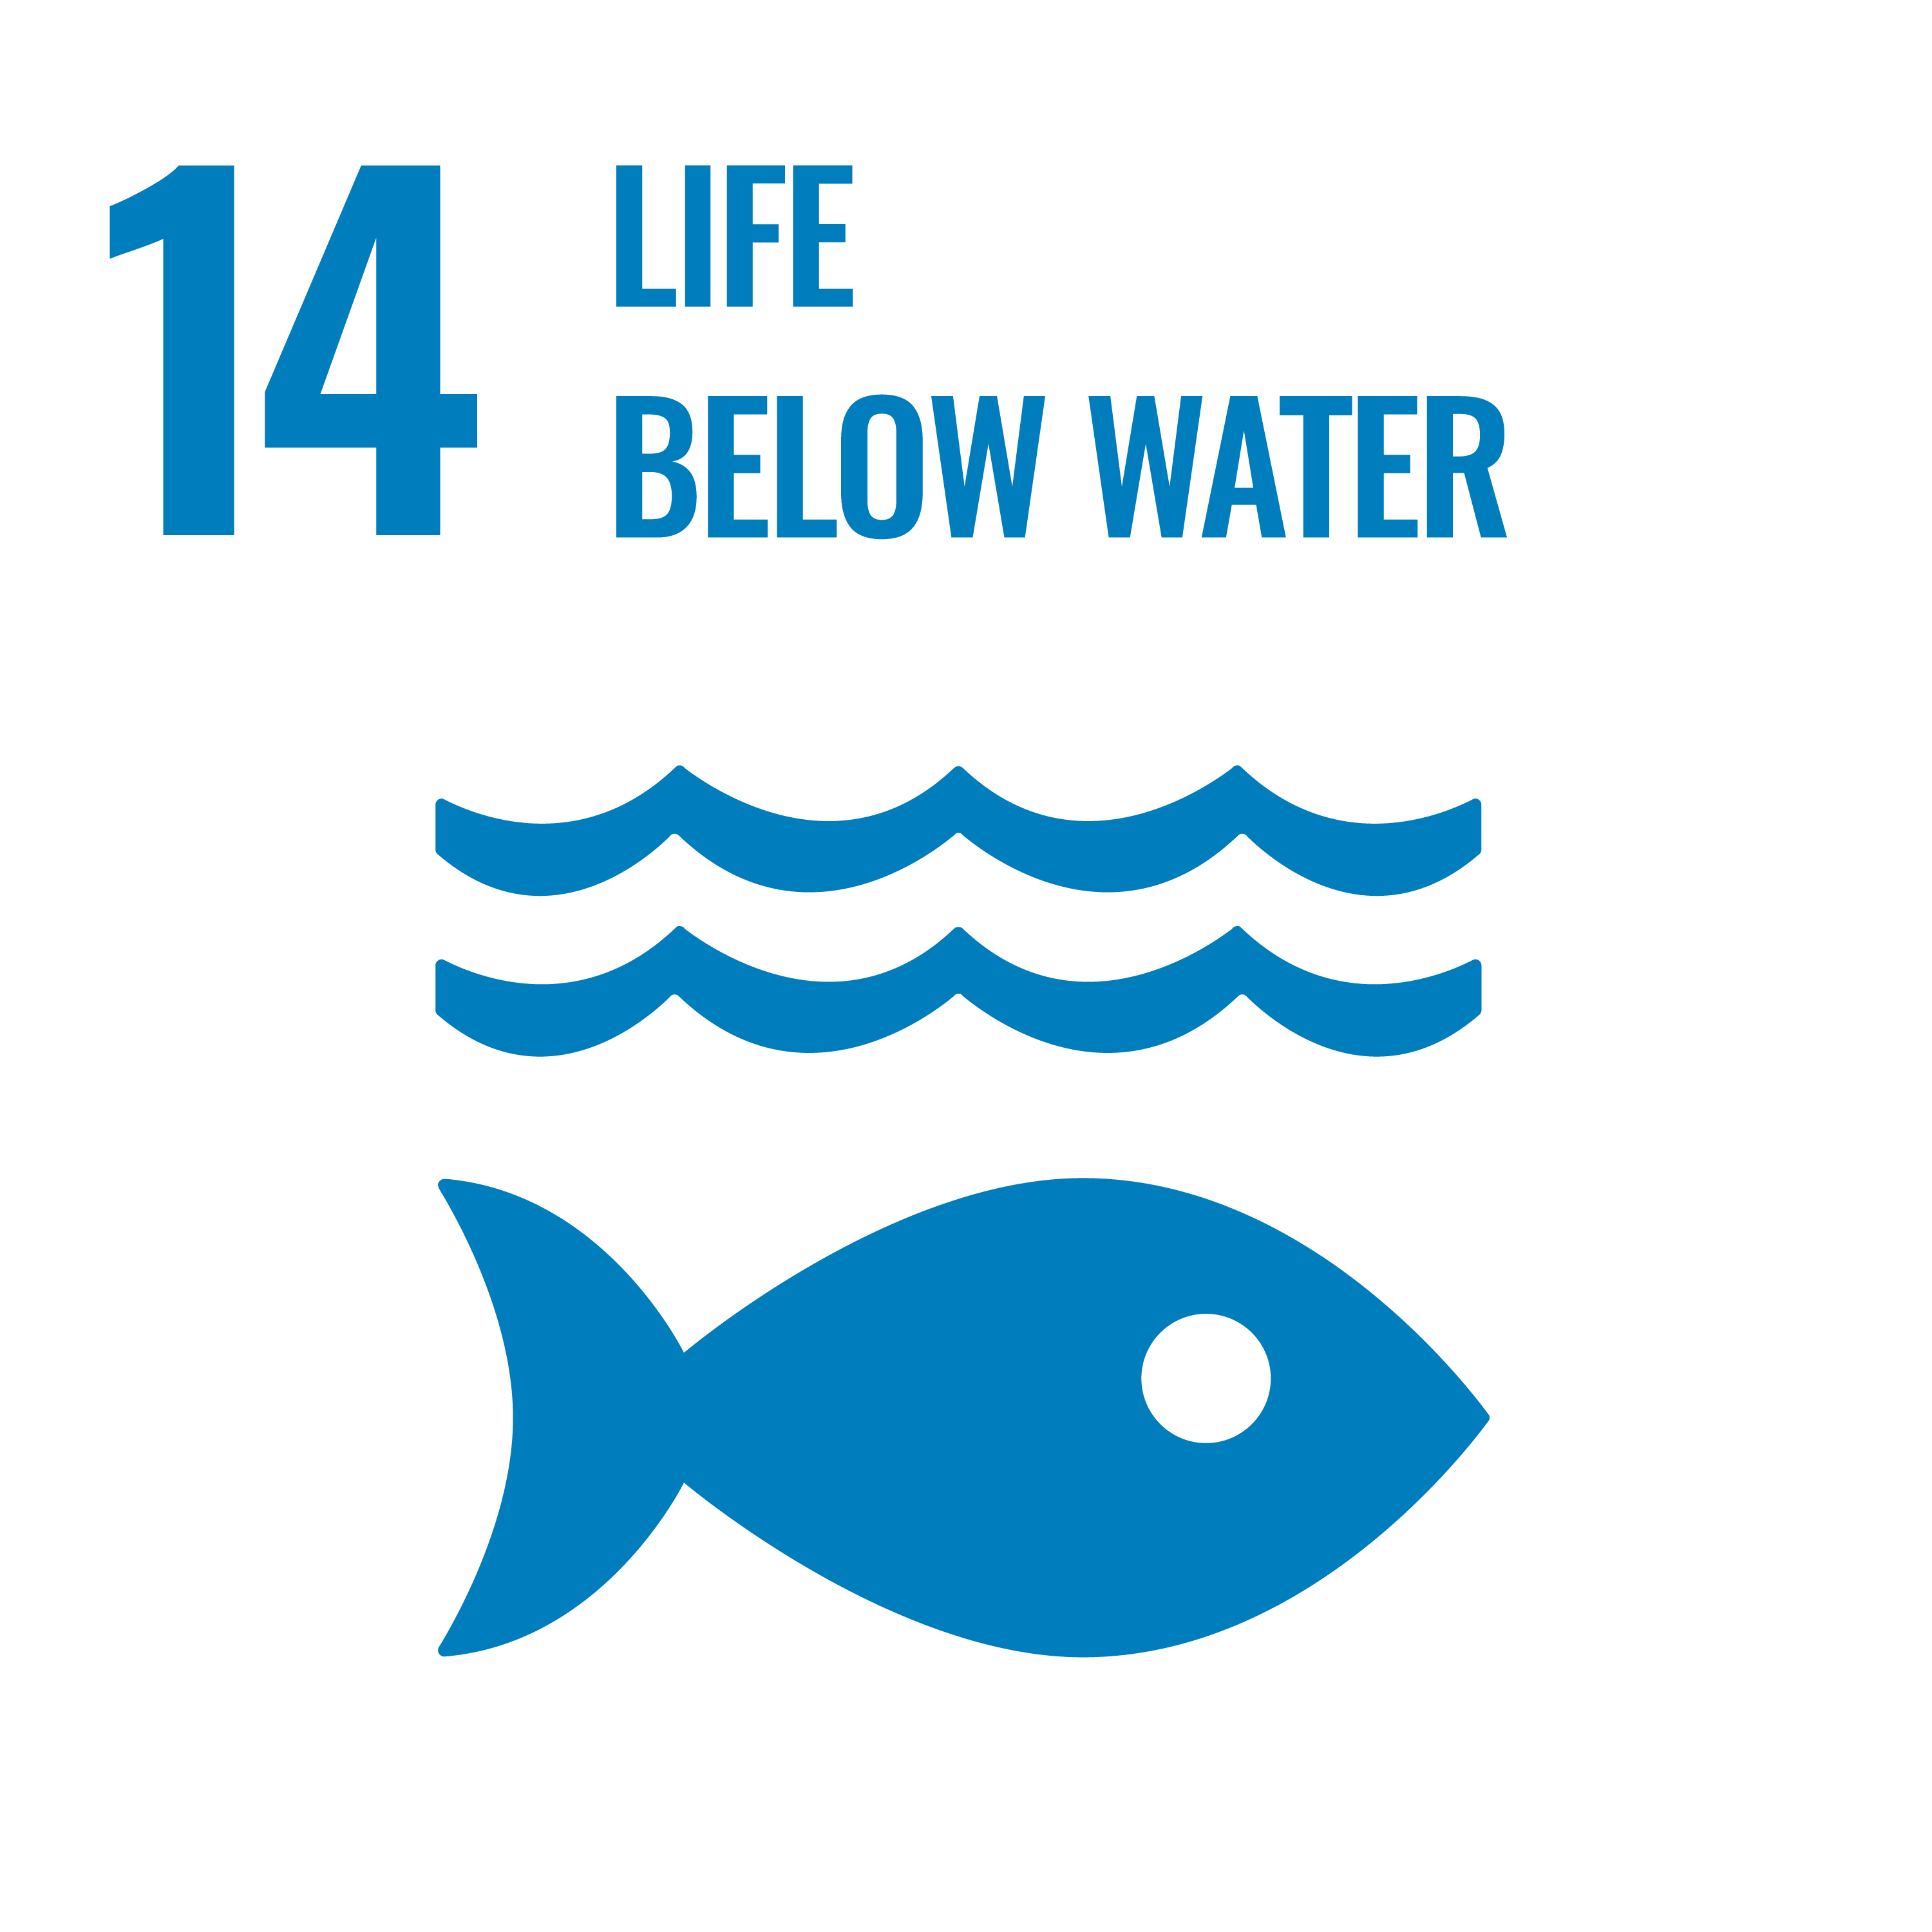
\includegraphics[width=\SDGsize]{Common/SDG_14_LifeBelowWater.png}~
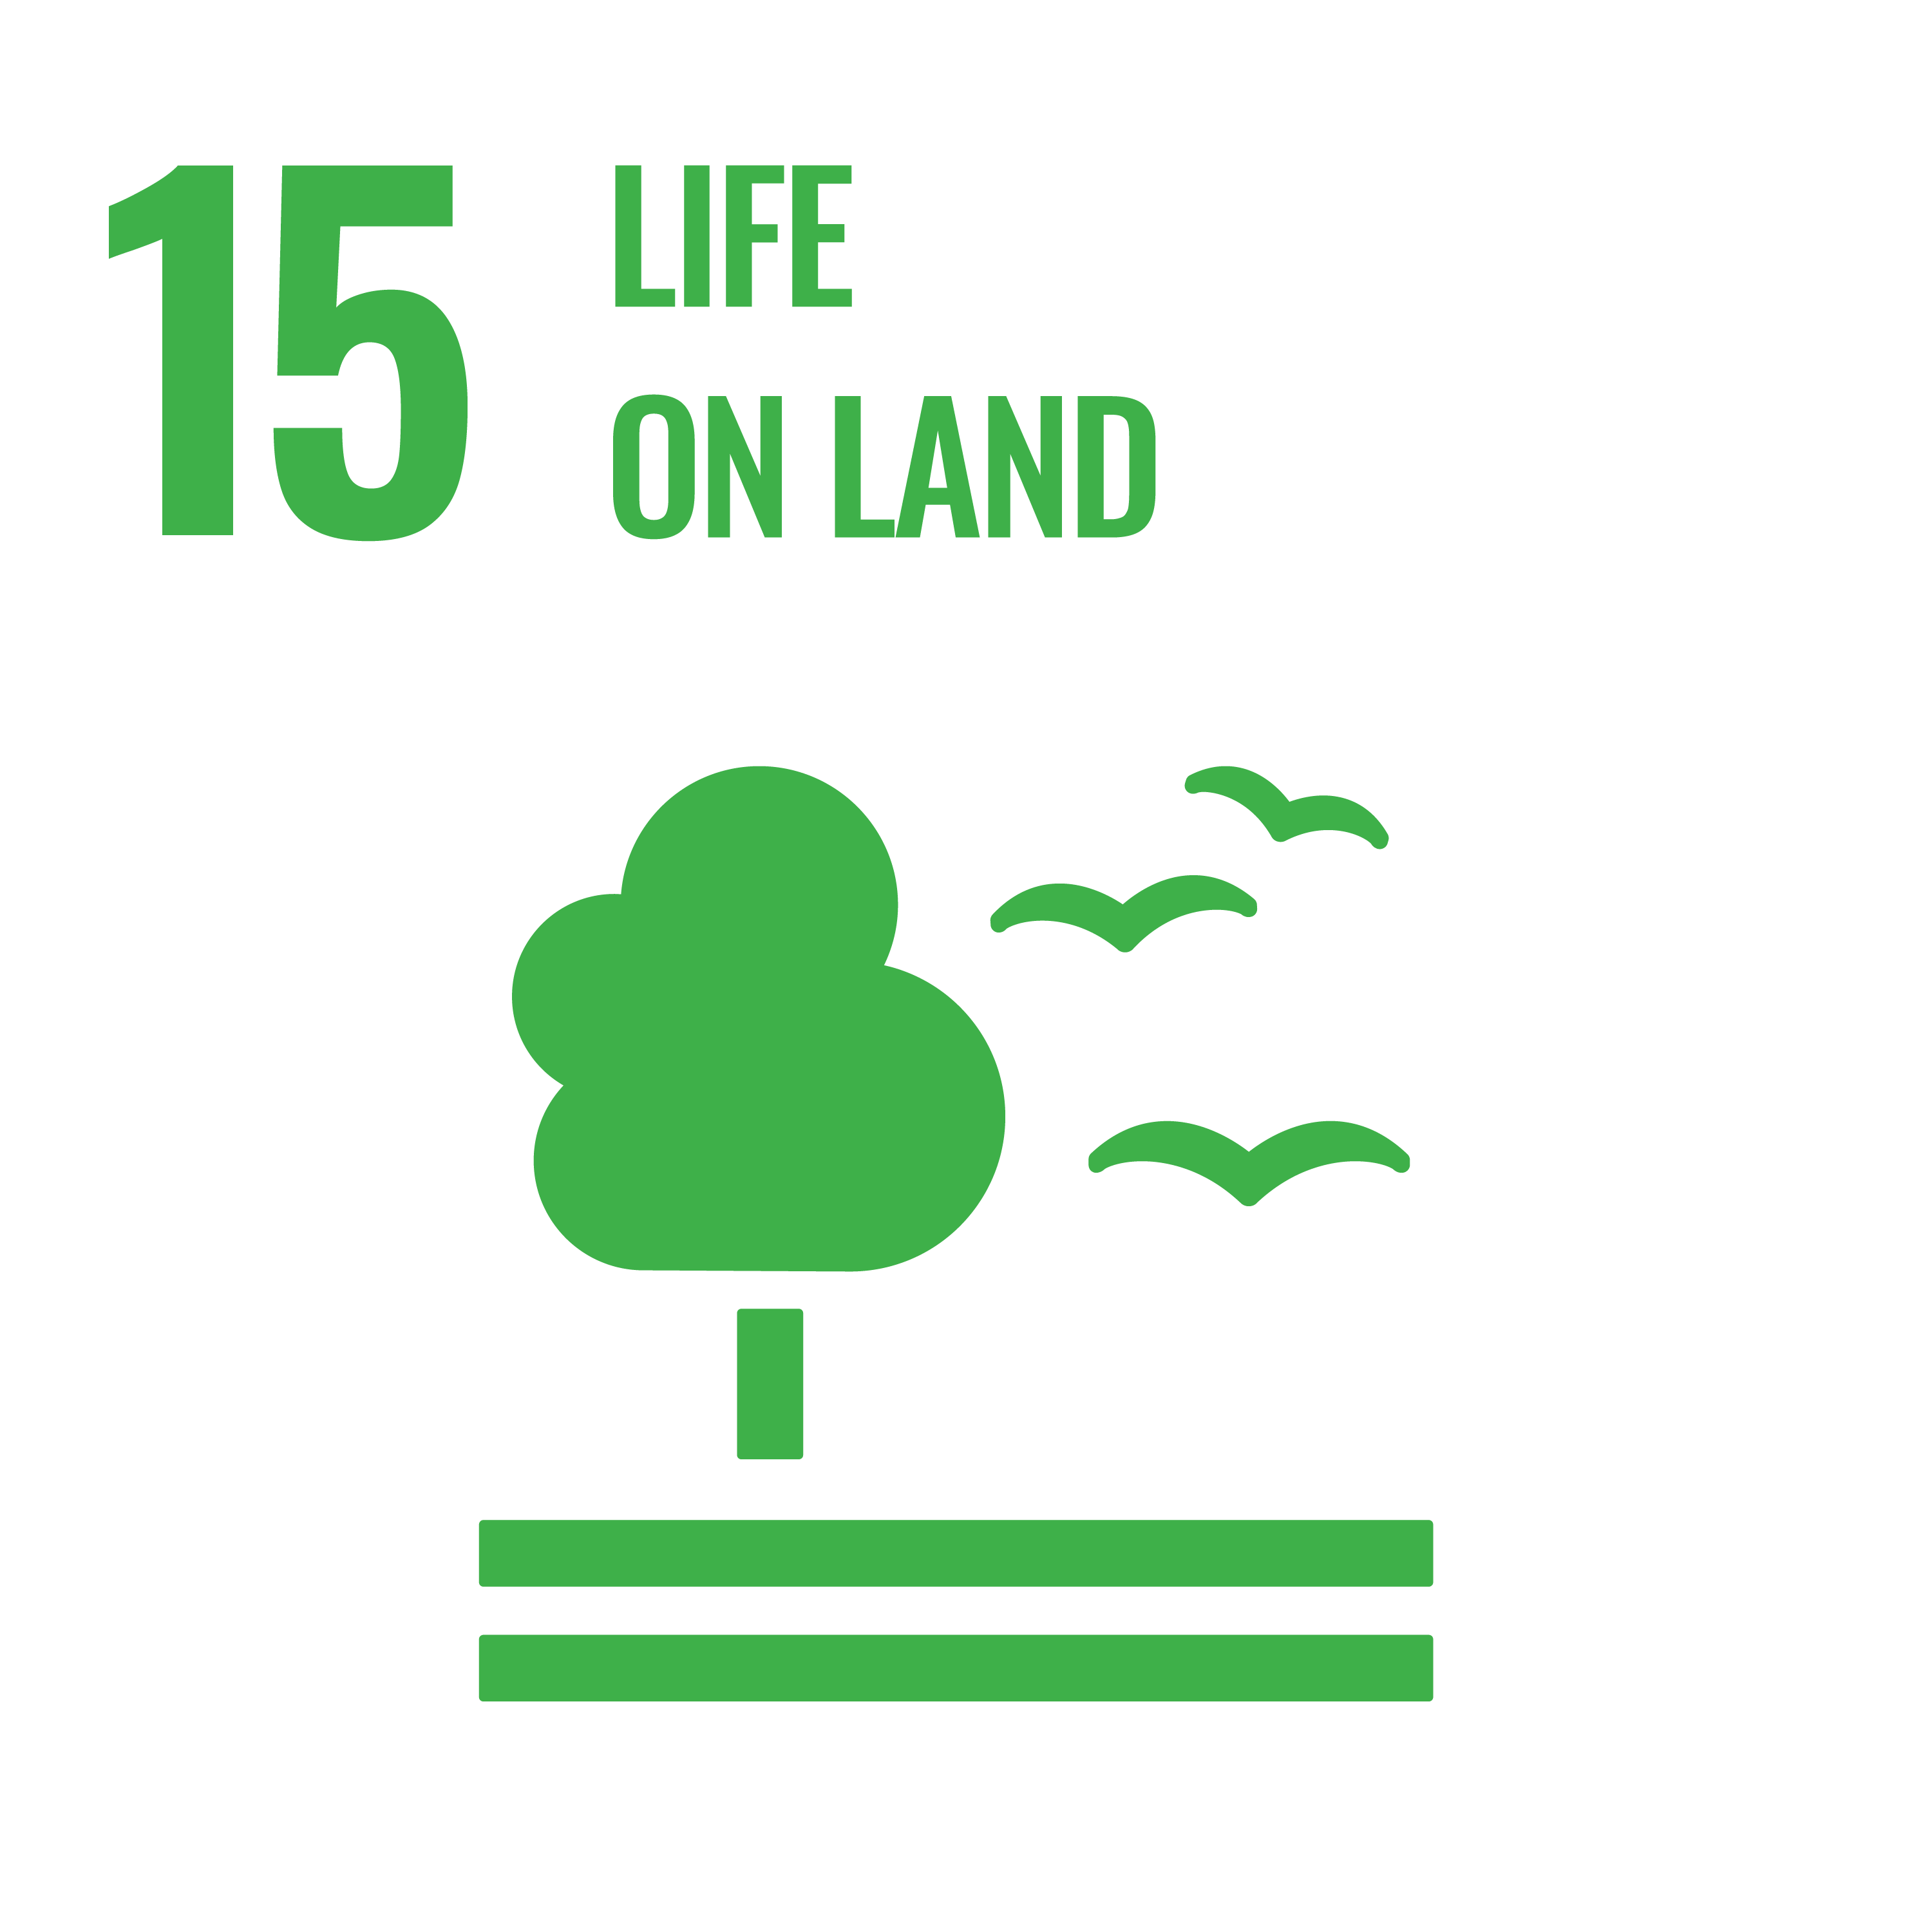
\includegraphics[width=\SDGsize]{Common/SDG_15_LifeOnLand.png}
\end{figure}

%%%%%%%%%%%%%%%%%%%%%%%%%%%%%%%%%%%%%%%%

\exSum

\noindent Half of the world's \acrshort{ghg} emissions, and over 90\% of global water stress and biodiversity loss events, are due to the extraction and processing of raw materials~\cite{EURaw}. Although most extracted materials are slated for the energy or agriculture sectors, the small fraction associated with consumption of goods and services is responsible for 18\% of EU emissions~\cite{EURaw}. Mitigating the climate impacts of the extraction, processing and trade of raw materials is a priority for the resilience of the EU~\cite{EURaw}, and it should also be a priority for the world climate agenda.

The generation of waste is a direct consequence of material consumption, and is aggravated by constraints in production, distribution, usage and repair, and disposal or recycling of consumables. Waste has severe impacts on life on land and at sea, often destabilizing local ecosystems.  It also damages the global ecosystem by contributing to climate change. Accumulations and inefficient disposal of waste products can result in pollution of ground water and air, thus directly affecting the health of individuals and communities at a large cost to society in terms of disease burden and lives lost. 

In an attempt to curb the footprint of waste generation, the concept of a circular economy has been  proposed~\cite{CircularEconomy}.  Any such proposal must be established in parallel with a will to reduce waste at source through sustainable procurement, repair and reuse, and used only as a transitional measure. Even a fully circular economy has some dissipation, and signatures of this energy waste need to be independently addressed and reduced~\cite{Forbes,SocialEurope,WRI}.

Procurement accounts for almost two-thirds of annual emissions at \acrshort{cern} \cite{CERNTownHall}, with a GHG footprint of the same order as its direct emissions in 2018, when the LHC was running \cite{Environment:2737239}. Although not yet fully included in reporting by other \ACR\ institutions, the environmental cost of procurement is likely proportionately large elsewhere.  Maximising the sustainability of the use cycle of resources should be a priority of the \ACR\ community. 

This section covers sustainable sourcing in \sref{subsec:Resources}, and reduction and treatment of waste, including E-waste, in \sref{subsec:Waste}. The use of materials in research infrastructure is also discussed in Section~\ref{sec:Technology}.

%%%%%%%%%%%%%%%%%%%%%%%%%%%%%%%%%%%%%%%%

\clearpage
\begin{reco2}{\currentname}
{
\begin{itemize}[leftmargin=3.5 mm]
\setlength{\itemsep}{\recskip}
\item Limit purchases and consider environmental credentials such as repairability and recyclability of products in purchasing decisions.

\item Service appliances regularly; share, repair, reuse and refurbish to minimise waste; sort and recycle.

\item Read the sections on computing (\sref{sec:Computing}), energy (\sref{sec:Energy}), food (\sref{sec:Food}), and research infrastructure and technology (\sref{sec:Technology}).
\end{itemize}
}
{\begin{itemize}[leftmargin=3.5 mm]
\setlength{\itemsep}{\recskip}
\item Adopt life cycle assessments and associated tools to assess environmental impact of all activities.

\item Institute sustainable purchasing, usage and end-of-life policies in the management of group consumables,  office supplies and single-use plastics \eg in conference events (see also Section~\ref{sec:CateringTableware} and Best Practice \ref{bp:PlasticFreeConf}).
\end{itemize}
}
{
\begin{itemize}[leftmargin=3.5 mm]
\setlength{\itemsep}{\recskip}
\item Prioritise suppliers instituting sustainable sourcing and operating policies, with a particular focus on the raw materials processing stage (see Best Practice~\ref{bp:SustainableRawMaterials}) and with the aim of creating demand for recycled (secondary) raw materials.

\item Provide an institutional pool of infrequently-used equipment to avoid redundancy in purchasing.

\item Proceduralise and prioritise repair of equipment, and enable through provision of tools and know-how.

\item Assess waste generation and management for the design, operation and decommissioning of IT and infrastructure projects by right-sizing needs, establishing specific treatment channels for all waste categories, and setting recycling targets that include the recycling of all construction waste, see, \eg \bpref{bp:HERAShieldingBlocks}.

\end{itemize}
}
\end{reco2}


%%%%%%%%%%%%%%%%%%%%%%%%%%%%%%%%%%%%%%%%
\subsection{Resources}
\label{subsec:Resources}

\ACR\ research can be resource-intensive, particularly in the building and maintenance of the often large experiments that drive progress in our fields.  These resources have an environmental impact over their entire life cycle, due to extraction of the raw materials used in their manufacture, their production and use, and their disposal once they become unusable or obsolete. Of these, the raw materials processing stage has been highlighted as having the greatest potential for emissions reduction (see, \eg Figure 2 of Ref.~\cite{EURaw}).  

The extraction of raw materials has important and extensive environmental costs~\cite{Dolega:2016}, mostly associated with the mining industry.  Acid mine drainage is the overriding problem and is a serious threat to water resources.  It results from water flow over ore creating sulphuric acid and leaching heavy metals from surrounding rock, thus contaminating groundwater and soil.  Mining operations can also deplete water resources, particularly in regions of limited water supply, severely restricting the availability of water to local consumers.  Fine particles and dust produced during mining operations and dispersed by winds affect air quality, and mining and its infrastructure leads to loss of agricultural land and even entire ecosystems through contamination or destruction of soil cover. Mining is the world's largest producer of waste, with copper, zinc, bauxite and nickel mining generating the largest ratios of waste to mined metal.  Disposal or storage of tailings, the waste products remaining after the extraction of valuable material from ore, is a major problem. These can be radioactive, and are sometimes illegally disposed of directly into rivers or seas.  Even when stored `responsibly' in tailings dams, incorrect geological siting of these dams, in tectonically active zones or regions of high rainfall, can lead to catastrophic loss of life and usable land~\cite{SILVAROTTA2020102119}.

Environmental sustainability aside, mining has a poor safety and human rights record~\cite{ResponsibleMiningIndex}, and is sometimes subject to dubious financing~\cite{MiningandMoneyLaundering}.  Mining of `conflict minerals', such as tin, tungsten, tantalum and gold, used in mobile phones and other everyday products, are sometimes used to finance armed conflict~\cite{EUConflictMinerals}.  

Sustainability regulations, both externally imposed and voluntary, are slowly being incorporated into the raw materials supply chains (see,\eg the Voluntary Principles on Security and Human Rights~\cite{VoluntaryPrinciples}), albeit slowly, and in an inconsistent and sometimes superficial manner~\cite{ResponsibleMiningIndex,ResponsibleMiningFoundation}.  For examples of sustainability initiatives, in particular in relation to raw materials supply chains, see~\bpref{bp:SustainableRawMaterials}.

An analysis of components used inside a smartphone and their impacts can be found in~Ref.~\cite{fairphone}.  Smartphone manufacturer Fairphone, for instance, sustainably sourced 56\% of 8 of the materials used in its phones in 2020, and have a set a target of fair sourcing of 70\% of 14 materials by 2023~\cite{fairphone2}. 

A ranked list of mined metals by overall environmental impact can be found in Table~\ref{tab:MetalImpact}.  This table was taken from the EU Raw Materials Information System~\cite{EURMIS}, with source data from Ref.~\cite{UNEP2010}.  Sourcing recycled metal from scrap produces significantly lower emissions.  Secondary aluminium, for example, was reported by the European Aluminium Association to emit 95\% fewer GHGs than primary production~\cite{EURaw}. Other materials used in \ACR\ experiments (\eg cobalt for magnets, rare earths for permanent magnets, niobium) are produced under very difficult conditions, with a high environmental or societal cost~\cite{FARJANA2019150, EURare, ALVES2019275}.  Formal discussions of their use and impact have already begun in the \ACR\ community, most recently at a workshop on Rare Earth Elements organised by \acrshort{ifast} at \acrshort{desy}~\cite{DESYRareEarth}.

\bigskip
{\centering
\ra{1.1}
\captionsetup{type=table}
\begin{tabular}{@{}lll@{}}\toprule
Ranking& Impact per kg & 
Impact global production \\ 
\midrule
1 & Palladium & Iron \\
2 & Rhodium & Chromium \\
3 & Platinum & Aluminium \\
4 & Gold & Nickel \\
5 & Mercury & Copper \\
6 & Uranium & Palladium \\
7 & Silver & Gold \\
8& Indium & Zinc \\
9 & Gallium & Uranium \\
10 & Nickel & Silicon \\

\bottomrule
\end{tabular}
\caption[Environmental impact associated with primary metals]{Environmental impact associated with primary metals, ranked by impact per kg, and total impact due to global production.  Taken from Ref.~\cite{EURMIS}, with material from Ref.~\cite{UNEP2010}.}
\label{tab:MetalImpact}
}


\subsubsection{Life cycle assessment}

Best practices in sustainable use and disposal of resources begins with a life cycle assessment (LCA): a cradle-to-grave accounting of all the environmental impacts of a resource.  As an example the ISO 14040 ~\cite{ISO14040} and ISO 14044~\cite{ISO14044} standards provide a systematic procedure for the analysis. Depending on the goal and scope of the analysis, the life cycle inventory comprises the quantification of all input and output flows. This includes raw materials, consumables, energy, products, waste, emissions, and groundwater and soil contamination. There are online tools and auditing agencies who provide help with the analysis, see, \eg Ref.~\cite{ProBasSi}.  For an LCA of a silicon wafer used in particle detectors, see \bpref{bp:SiWafer}.

\subsubsection{Sustainable sourcing \label{sec:sustainablesourcing}}

Purchasing policy can have a major impact on the environmental costs of procurement. 
The \ACR\ community should prioritise suppliers that implement sustainable thinking , sourcing,  and operation. This could include voluntary provision of life cycle assessments for their products (see above), or certification of, \eg proof of origin.
Sustainability requirements on suppliers could also be incorporated into tenders and purchasing regulations, allowing these considerations to be weighed in tandem with cost in the tendering process.  Since much of \ACR\ funding is public, purchasing regulations, which are influenced by funding agencies, an additional important stakeholder in this process, must be reassessed.  For examples of best practice in sustainable procurement, see~\bpref{bp:SustainableRawMaterials}.  A strategic approach to sustainable purchasing has been outlined in ISO 20400~\cite{ISO20400}.  

CERN is in the process of defining a new environmentally responsible procurement policy, to be implemented in 2023~\cite{Hartley}.  Key measures being considered include requiring sustainability certification from suppliers, with a focus on those with highest potential to drive sustainability issues~\cite{Hartley}.  For further sustainable procurement and waste policies being explored by CERN, see~\bpref{bp:CERNSustainableProcurement}.  

\begin{bestpractice}[\label{bp:SustainableRawMaterials}Sustainability in raw materials supply chains\\{\noindent\footnotesize Contribution from Enrico Cennini, IPT (Industry, Procurement and Knowledge Transfer), CERN, summarised from Ref.~\cite{EURaw}}.]{Sustainability in raw materials supply chains}%
\noindent Sustainable procurement requires sustainability in all phases of the supply chain, from producers to processors and traders.  Hallmarks of sustainability among suppliers include the following (with the relevant phase(s) shown in parentheses):
\begin{itemize}
    \item Compliance with sustainability standards set and certified by non-profit, multi-stakeholder organizations. (Producers, processors, traders) \\\vspace{-0.1in} 
    {\small \eg Aluminium Stewardship Initiative, Responsible Steel certification, Responsible Jewelry Council (precious metals, stones).}
    \item Voluntary implementation of certified energy- and environmental-management systems, such as ISO 50001 and ISO 14001. (Producers, processors, traders)  
    \item Setting of voluntary sustainability targets by sectoral industry associations. (Producers, processors, traders) \\
    {\small \eg steel-making industry and ammonia producers investigating low-carbon sources of hydrogen for imminent adoption.}
    \item Demonstrable investment in technological solutions for improving energy efficiency of operations, such as employing `Best Available Techniques' (BATs) and keeping to `Associated Environmental Performance Levels' (BAT-AEPLs). (Producers, processors, traders) \\ 
    {\small \eg transition to lower carbon sources for power supply, implementation of `ventilation-on-demand' (gold and potash mining); replacing diesel fleet with hybrid electric, innovative and energy efficient loading and haulage systems (mining); continuous monitoring and improvement of transportation methods.}
    \item Requiring third-party verified sustainability certificates from upstream suppliers. (Processors, traders) \\
    {\small \eg some aluminium manufacturers; selected wood and copper processors' business partner code of conduct encodes supplier sustainability requirements.}
\end{itemize}
\end{bestpractice}

\begin{bestpractice}[\label{bp:CERNSustainableProcurement}CERN sustainable procurement and waste policy\\{\noindent\footnotesize Contribution by Quentin Salvi, Waste Management Project Coordinator, CERN.}]{CERN sustainable procurement and waste policy}%
\noindent Avenues being actively explored by CERN to improve sustainability in procurement and waste include the following:
\begin{itemize}
    \item Implementing a circular economy, both internally and externally.      
\item Knowledge-sharing with partners and the local authority. 
\item Consolidation of CERN equipment, 
behavioural change in industrial practices and management. 
\item Optimisation of services based on CERN data. 
\item User-awareness.
\end{itemize}
\end{bestpractice}

\subsection{Waste}
\label{subsec:Waste}
Around 3\% of global GHG emissions is due to solid waste disposal, the organic component of which decomposes in wastewater and landfills, producing methane and nitrous oxide~\cite{owidco2andothergreenhousegasemissions}.  This is despite a 60\% decrease in the amount of waste landfilled in the EU in the past two decades, due partly to an increased legislative focus on alternative treatment methods, such as recycling and composting, as well as more widespread landfill gas recovery~\cite{Eurostat}.

The fastest-growing portion of EU waste output is E-waste~\cite{EUNews}: powered products with electrical components that are discarded into the waste stream. In addition to releasing hazardous
chemicals into the environment, improperly treated E-waste contributes to global warming through failure to recuperate valuable mined materials, and direct release of GHGs including refrigerants (see \fref{fig:ewaste} for statistics on global E-waste generation and disposal in 2019). Moreover, E-waste can often be shipped illegally to developing countries without infrastructure for safe recycling~\cite{Forti2020, OECDLib}. Exploding demand for digital devices, fuelled by their fast obsolescence and difficulty to repair, has also given rise to a boom in the mining industry.  This boosts the economy in resource-rich countries, where working conditions are usually unsafe and unpleasant, and causes deforestation and pollution~\cite{OECDLib}.

Increasing the life-span of consumer electronics through more comprehensive right-to-repair 
legislation is an integral part of the EU's strategy for a circular economy~\cite{EUNews,EUR2RSummary}.  According to a 2018 European Commission study, however, the cost of repair was the most frequent reason consumers chose to replace four common household electrical and electronic goods~\cite{ECConsumerStudy}. 
Right-to-repair advocates are pushing for more comprehensive and far-reaching legislation, including policies that will empower consumers to make simple repairs themselves, as well as government incentives to repair through, \eg financial aid~\cite{R2RPolicy}. A trial scheme for the latter has already been implemented in France~\cite{FrenchRepairAid}.  Unfortunately, today's legislation is formulated piecemeal and is slow to take effect.  In addition to instituting sustainable purchasing, use and de-inventorising/disposal policies for electrical and electronic goods (see Recommendations), \ACR\ institutions could encourage the sustainable use of personal electronic devices by making repair equipment freely available, with guidance from experts on a volunteer basis.

\begin{figure}
    \centering
    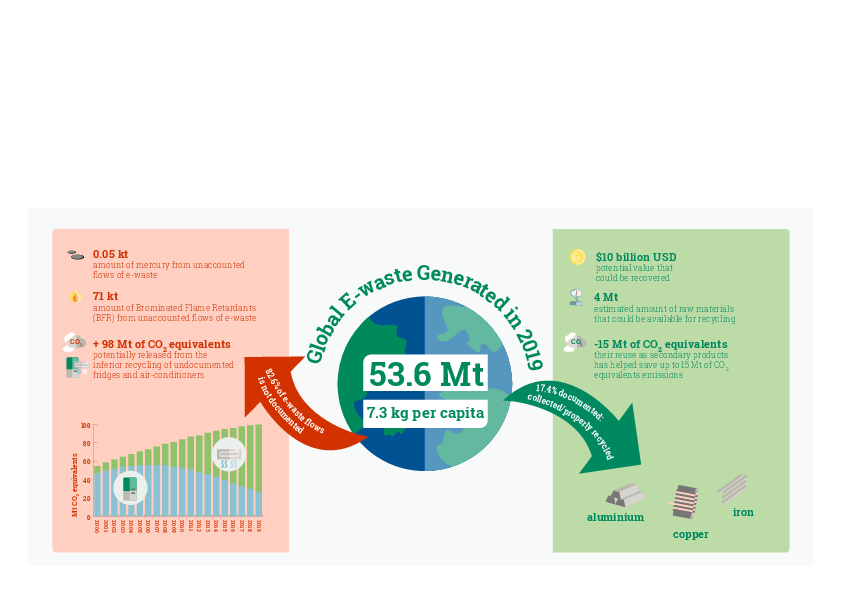
\includegraphics[width=0.9\textwidth]{Sections/Figs/Waste/EWaste-1.png}
    \caption[Global E-waste generated in 2019]{The generation of global E-waste in 2019. About 83\% of E-waste goes undocumented, highlighting the importance of its re-use and recycling. Figure reused from Ref.~\cite{EWaste} under the terms of the \href{https://creativecommons.org/licenses/by-nc-sa/3.0/igo/}{Creative Commons Attribution-NonCommercial-ShareAlike 3.0 IGO (CC BY-NC-SA 3.0 IGO) license}.\label{fig:ewaste}}
\end{figure}

%%%%%

\begin{bestpractice}[Re-purposing shielding blocks\label{bp:HERAShieldingBlocks}]{Re-purposing shielding blocks}%
\noindent Initially, the heavy concrete blocks in the HERA halls had served
as protection against radiation. Five hundred of these discarded shielding blocks were stored, unused,  for years on the DESY campus in Hamburg, Germany. 6,000 tonnes of this heavy concrete were shredded in 2020. The concrete rubble is already being used as a new building material for campus renovations~\cite{DESYsustainableReport2022}.
\end{bestpractice}

\subsubsection{Plastic Waste}
Plastic is a versatile product, efficient, cheap, stable, and infinitely mouldable.  Its unique properties have resulted in our increasing reliance on it over decades, making it very hard to live without. 

GHG emissions from production, use and disposal of conventional (fossil-fuel-based) plastics is significant, and growing.  It is expected to increase to $\sim$2.1 \acrshort{tco2e} per capita by 2040, accounting for almost 20\% of the global carbon budget~\cite{UNPollutionSolution}.  Less than one tenth of plastic waste produced to date has been recycled, with the remainder being landfilled or incinerated~\cite{UNPollutionSolution}.  This plastic waste contaminates the natural environment.  It is slow to degrade (biodegradable plastics included), releasing potentially harmful chemicals into the environment in the process, eventually breaking down to micro- and nano-plastic particles that infiltrate the food chain.  Microplastics are also found in waste water, due to washing of synthetic textiles, and in cosmetic and personal care products~\cite{Microplastics}.  The health impacts of ingested plastic waste are not yet completely understood, but they are thought to alter metabolic pathways and hormone signalling in animals.

A simple ban on single-use plastics, and plastics that are not at least 99\% recyclable would greatly limit microplastic pollution. 

\subsubsection{Conference Waste\label{sec:ConferenceWaste}}

The amount of waste generated at conferences can be significantly reduced by replacing printed timetables and welcome packs with a well-designed conference app, see, \eg Whova~\cite{Whova}, and keeping conference gifts digital (\eg e-vouchers/discounts for local restaurants or activities).    Sustainable stationery should be distributed on a need-only basis, and banners, posters and name tags made plastic-free and reusable.  For waste-minimising initiatives implemented at the plastic-free 2019 conference of the Australian Marine Society, see~\bpref{bp:PlasticFreeConf}.  For sustainability concerns in conference catering, see Section~\ref{sec:CateringTableware}.


\begin{bestpractice}[Plastic-free 2019 conference of the Australian Marine Sciences Association\\
{\noindent\footnotesize Taken from Ref.~\cite{PlasticFreeConf}}\label{bp:PlasticFreeConf}]{Plastic-free conference, Australian Marine Sciences Association}%
\noindent In response to the growing problem of plastic pollution, the Australian Marine Sciences Association undertook to make their 2019 conference 100\% plastic free. Concrete measures they implemented for their roughly 600 delegates included:
    \begin{itemize}
        \item plastic-free cardboard name badges with bamboo lanyards and metal clips
        \item complimentary fabric tote bags with conference logo
        \item no printed envelopes for registration packs, no printed conference abstracts
        \item any printing necessary was done on sustainably-sourced paper, using a solar-powered printer
        \item sustainably-sourced pencils instead of pens, with sharpening stations provided
        \item no packaged sweets
        \item delegates were asked to bring reusable water bottles, or pre-register to buy them at the conference
        \item water jugs with glassware provided at back of each presentation room
        \item reusable, washable plates, cups silverware and glassware for all meal and coffee breaks
        \item vegetarian catering for tea breaks
    \end{itemize}
    These measures were implemented without affecting the budget, although some solutions reportedly took significant planning and forethought, and clear communication with the event organiser and providers.
\end{bestpractice}

\subsubsection{Catering Tableware}
\label{sec:CateringTableware}
A life-cycle analysis by the UN Environment Programme concludes that ``reusable tableware consistently outperforms single-use tableware in all the studies and across all environmental impact categories (with water use being the exception, because of washing). This type of analysis takes into account all the variables that affect the environmental impact of a product, from manufacturing to end-of-life treatment. The case for reusable tableware is strengthened in countries where renewable energy makes up a high proportion of the grid mix and where end-of-life treatment options are not well developed''~\cite{UNEP2021}. 

In outdoor or remote environments or ‘pop-up’ events with no fixed catering facilities, where reusable tableware is impractical, single-use biodegradable tableware is preferable to other single-use tableware if it is industrially composted mixed in with food waste~\cite{UNEP2021}.\footnote{Industrial composting of household food waste is currently not the norm in most geographical locations within the USA~\cite{EPAWasteFoodMgmt}, and many existing industrial composters do not accept biodegradable plastic waste~\cite{BioplasticsAtIndustrialSites}.} 

Unlike emissions due to reusables, which are dominated by their use phase due to repeated washing, the  main impact of biodegradable tableware is due to its production. For conventional plastic, a significant role is also played by end-of-life management.  Quantitative analysis of their relative emissions is thus strongly dependent on assumptions about manufacture and disposal, including the material demand.  On the practical side, to minimise this impact when planning conference catering one should always choose the lightest-weight disposable tableware fit for purpose, preferably manufactured in a country with a significant proportion of renewables in its energy and electricity mix.  For a comparison of emissions due to different choices of disposable catering tableware for pop-up catering, see~\csref{cs:conferencetableware}.

\begin{casestudy}[Comparing tableware for pop-up catering\label{cs:conferencetableware}]{Comparing tableware for pop-up catering}%
\noindent The production and disposal of single-use tableware has a significant impact across all environmental factors, including acidification, eutrophication, human health, land use and water depletion.  However we will focus here only on its GHG emissions.
%as the most urgent issue facing us today, and the one with the most reliable and robust indicators for decision making.

    We will consider for benchmarking purposes a large-scale conference with 1,000 attendees and informal lunchtime catering (\ie with no dishwashing capability), and compare the life-cycle emissions due to tableware made from conventional plastics, which are disposed of by a combination of incineration and landfill according to the European average (presumed food remnants making them unsuitable for recycling), and from biodegradable bioplastics, which are industrially composted along with the food remnants.

    We assume each set of tableware consists of a dinner plate and cup, a knife and fork, and a paper napkin and tray mat, all manufactured to the same size and thickness, but with possible differences in weight due to their respective material densities.  A full list of assumptions and details of the analysis can be found in the original article~\cite{Fieschi2018}.   

    The total emissions for 1,000 sets of conventional polystyrene tableware is 221 kg \acrshort{co2e}, as compared with 109 kg \CdOe\ for the biodegradable bioplastic tableware, a saving of 112~kg \CdOe, around the emissions of a flight from Paris to Geneva.  
%Note that much of the comparative advantage of the bioplastics comes from their end-of-life treatment; their production is significantly more resource-intensive than conventional plastic tableware.  

%    It is difficult to compare these figures to those for reusable tableware, since reliable, peer-reviewed studies that allow quantitative comparison between all three types of tableware are hard to come by.  
    For the purposes of comparison, we include here the emissions cost of 1,000 dishes and cups from a 2015 study by Italian plastics company Pro.mo~\cite{PROMO2015}.  They put the total emissions due to reusables at 26 kg \CdOe, with the emissions due to conventional plastic dishes and cups (polypropylene in this case) at 79 kg \CdOe.
%\footnote{We do not quote their estimate for bioplastics, since they do not consider the composting of bioplastics, but rather assume they are disposed of by incineration and landfill, in a similar way to conventional plastics.}  
Note that these figures are specific to the electricity and energy mix of the European market, which has a large impact on the dominant emissions in all cases.
%: for production in the case of bioplastics, production and incineration for conventional plastics, and washing for reusables. 

\end{casestudy}

\end{document}